\documentclass[article]{IEEEtran}
%\usepackage{hyperref}
\usepackage{amsmath}
\usepackage{tikz}
\usepackage{cite}
\usepackage{circuitikz}
 \usepackage{tkz-euclide}
 \usetikzlibrary{angles}
 \usetikzlibrary{positioning}
\usepackage{tikz-3dplot}
\usepackage[utf8]{inputenc}
\usepackage{color}
\usepackage{soul}
\usepackage{amssymb}
\newcommand{\C}[1]{\mathbf{\hat{#1}}}
\newcommand{\M}[1]{\mathbf{#1}}
\newcommand{\T}[1]{\mathrm{#1}}
\newcommand{\V}[1]{\boldsymbol{#1}}
\newcommand{\TR}[1]{\color{red}#1\color{black}} 
\newcommand{\TB}[1]{\color{blue}#1\color{black}}
\newcommand{\AV}[1]{\bar{\bar{\V{#1}}}}
\newcommand{\bs}[1]{\boldsymbol{\V{#1}}}
\renewcommand{\u}[1]{\boldsymbol{\hat{#1}}}
\usetikzlibrary{shapes.symbols}
\newcommand{\Jh}{\hat{\T{J}}}
\newcommand{\Hhone}{\hat{\T{H}}^{(1)}}
\newcommand{\Hh}{\hat{\T{H}}^{(2)}}
\newcommand{\Hhp}{\hat{\T{H}}^{(2)\prime}}
\newcommand{\rbkind}{\chi}
\newcommand{\Xopchar}{P}
\newcommand{\Yopchar}{Q}
\newcommand{\Xop}{\mathcal{\Xopchar}}
\newcommand{\Xmat}{\mathbf{\Xopchar}}
\newcommand{\Yop}{\mathcal{\Yopchar}}
\newcommand{\Ymat}{\mathbf{\Yopchar}}
\newcounter{tempEQCounter}


\title{Scattering Properties of Spherical Time-Varying Conductive Shells}
\author{Kurt Schab, \IEEEmembership{Member, IEEE}, Bradley Shirley, \IEEEmembership{Student Member, IEEE}, and K.C. Kerby-Patel \IEEEmembership{Senior Member, IEEE}
\thanks{Manuscript received  \today; revised \today.}
\thanks{K. Schab and B. Shirley are with the Department of Electrical and Computer Engineering, Santa Clara University, Santa Clara, CA, USA (e-mail: kschab@scu.edu).}
\thanks{K. C. Kerby-Patel is with the Engineering Department, University of Massachusetts Boston, Boston, MA USA (e-mail: kc.kerby-patel@umb.edu).}}
\markboth{Journal of \LaTeX\ Class Files,~Vol.~XX, No.~XX, \today}{TBD: Short title }

\begin{document}

%\input{response-r2}
%\newpage
%\documentclass[12pt]{article}
\usepackage{amsmath}
\usepackage{enumerate}
\usepackage{xr}
%\externaldocument{epinet}
\newcommand{\fullspace}{\mathfrak{N}}

\pdfminorversion=4
\usepackage{url} 

\newcommand{\czero}{[C.1]}
\newcommand{\cone}{[C.2]}
\newcommand{\ctwo}{[C.3]}
\newcommand{\cthree}{\mbox{[C.4]}}
\newcommand{\cfour}{[C.5]}
\newcommand{\cfive}{[C.6]}

\newcommand{\ghoster}[0]{}

% OLD PREAMBLE:

% \usepackage{jsen}
% \usepackage{cite}
% \usepackage{amsmath,amssymb,amsfonts, bbm, mathtools}
% \usepackage{algorithm,algorithmic}
% \usepackage{graphicx}
% \usepackage{textcomp}
% \usepackage{wrapfig}
% \usepackage{xfrac}
% \usepackage{stackengine}
% \usepackage{subfigure}
% \def\delequal{\mathrel{\ensurestackMath{\stackon[1pt]{=}{\scriptstyle\Delta}}}}



% \usepackage{color, soul}
% \newcommand{\hlt}[1]{\hl{#1}}
% \newcommand{\red}[1]{\textcolor{red}{#1}}

% \def\BibTeX{{\rm B\kern-.05em{\sc i\kern-.025em b}\kern-.08em
%     T\kern-.1667em\lower.7ex\hbox{E}\kern-.125emX}}
% \markboth{\journalname, VOL. XX, NO. XX, XXXX 2017}
% {Author \MakeLowercase{\textit{et al.}}: Preparation of Papers for IEEE TRANSACTIONS and JOURNALS (February 2017)}
% \definecolor{abstractbg}{rgb}{0.89804,0.94510,0.83137}
% \setlength{\fboxrule}{0pt}
% \setlength{\fboxsep}{0pt}

% NEW PREAMBLE:


\usepackage{amsmath,amsfonts,amssymb,bbm, amsthm, xfrac}
\usepackage{algorithmic}
\usepackage{algorithm}
\usepackage{array, multirow}
% \usepackage[caption=false,font=normalsize,labelfont=sf,textfont=sf]{subfig}
\usepackage{caption, subcaption}
\usepackage{textcomp}
\usepackage{stfloats}
\usepackage{url}
\usepackage{verbatim}
\usepackage{graphicx}
\usepackage{cite}
\usepackage{caption}
\usepackage{subcaption}
\hyphenation{}

\theoremstyle{plain}
\newtheorem{theorem}{Theorem}

\usepackage{color, soul}
\newcommand{\hlt}[1]{\hl{#1}}
\newcommand{\red}[1]{\textcolor{red}{#1}}


\RequirePackage[letterpaper, portrait, margin=1in]{geometry}

\usepackage[]{natbib}
\bibpunct{(}{)}{,}{a}{}{,}

\renewcommand{\s}{\vspace{0.1cm}}

\setlength{\bibsep}{0pt plus 0.3ex}
\newcommand{\size}{L}
\newcommand{\norm}[1]{\lVert#1\rVert}

\def\baselinestretch{1.05}
\newcommand{\mQ}{\mathbb{Q}(\bbeta^\star, \bSigma)}
\newcommand{\tr}{\mathop{tr}}
\newcommand{\supp}{\mathbb{S}}
\newcommand{\wm}{\widehat{\rho}}
\newcommand{\btas}{\bta^\star}
\newcommand{\bepsilon}{\bm{\delta}}
\renewcommand{\interior}{\textnormal{int}}
\newcommand{\BBB}{\mathbb{B}}

\newcommand{\compl}{\mbox{comp}}
\renewcommand{\balpha}{a}
\usepackage{amsfonts,amsmath,amssymb,latexsym,bm,bbm}
\newcommand{\mbG}{\mathscr{G}}
\RequirePackage{amsthm,amsmath}
\usepackage{times}
\usepackage{natbib}
\hyphenation{neigh-bor-hood}
\newcommand{\deltaepsilon}{\delta(\epsilon)}
\renewcommand{\bta}{\bm{\eta}}
\renewcommand{\bta}{\bm{\eta}}
\usepackage{multirow}
\newcommand{\GG}{\mathscr{G}(\omega)}
\newcommand{\HH}{\mathscr{G}(\omega_1)}
\usepackage{mathtools}
\newcommand{\comp}{\mbox{comp}\,}
\renewcommand{\one}{\mathbbm{1}}
\renewcommand{\mM}{\mathbb{M}}
\newcommand{\mMs}{\mM(\omega)}
\newcommand{\etaspace}{\bm{\Xi}}
\renewcommand{\mT}{\mathbb{T}}
\usepackage[mathscr]{eucal}
\renewcommand{\bmu}{\bm{\mu}}
\renewcommand{\bA}{\bm{A}}
\renewcommand{\bt}{\bm{t}}
\renewcommand{\bB}{\bm{B}}
\renewcommand{\bC}{\bm{C}}
\renewcommand{\norm}[1]{\lVert#1\rVert}
\renewcommand{\mbR}{\mathbb{R}}
\renewcommand{\lip}{{\tiny\mbox{Lip}}}
\renewcommand{\lte}{&\leq&}
\renewcommand{\gte}{&\geq&}
\renewcommand{\mD}{\mathbb{D}}
\renewcommand{\btheta}{\bm{\theta}}
\renewcommand{\bTheta}{\bm{\Theta}}
\newcommand{\bThetas}{\bm{\Theta}^\star}
\renewcommand{\tends}{\to}
\renewcommand{\tend}{\rightarrow}
\newcommand{\rint}{\mathop{\mbox{rint}}}
\renewcommand{\su}{\sup\limits}
\renewcommand{\mS}{\mathbb{S}}
\renewcommand{\mbX}{\mathbb{X}}
\renewcommand{\mbY}{\mathbb{Y}}
\renewcommand{\uu}{x_i}
\renewcommand{\vv}{x_i^\star}
\renewcommand{\logit}{\mbox{logit}}
\renewcommand{\tv}{{\tiny\mbox{TV}}}
\renewcommand{\mbV}{\mathbb{V}}
\renewcommand{\mB}{\mathscr{B}}
\renewcommand{\BB}{\mathscr{B}}
\renewcommand{\CC}{\mathscr{C}}
\usepackage{bbm,amsfonts,graphicx}

\newcommand{\xk}{\bm{x}_k}
\newcommand{\yk}{\bm{y}_k}
\newcommand{\Xk}{\bm{X}_k}
\newcommand{\Yk}{\bm{Y}_k}
\newcommand{\mXk}{\mX_k}
\newcommand{\mYk}{\mY_k}
\newcommand{\mSS}{\mathbb{S}}
\newcommand{\ppp}{m}
\newcommand{\qqq}{q}
\newcommand{\diminf}{\ppp}
\usepackage{multicol}
\renewcommand{\vec}{\mathop{\mbox{vec}}}
\newcommand{\conv}{\mbox{conv}}
\renewcommand{\bx}{\bm{x}}
\renewcommand{\=}{&=&}
\renewcommand{\hide}[1]{}
\newcommand{\ghost}[1]{}
\renewcommand{\zs}{\bm{z}^\star}
\newcommand{\Thetad}{\Theta_0}
\newcommand{\bthetas}{\btheta^\star}
\newcommand{\thetas}{\theta^\star}
\newcommand{\thetad}{\thetas}
\newcommand{\etas}{\eta^\star}
\newcommand{\bthetad}{{\btheta}_0}
\newcommand{\bThetad}{{\bTheta}_0}
\newcommand{\thetah}{\widehat{\theta}}
\newcommand{\bthetah}{\widehat{\btheta}}
\newcommand{\bthetahh}{\widehat{\bthetah}}
\renewcommand{\mX}{\mathbb{X}}
\renewcommand{\mbT}{\mathbb{T}}
\renewcommand{\mC}{\mathbb{C}}
\renewcommand{\mY}{\mathbb{Y}}
\renewcommand{\mI}{\mathbb{I}}
\renewcommand{\mZ}{\mathbb{Z}}
\renewcommand{\be}{\begin{equation}\begin{array}{lllllllllllllllll}}
\renewcommand{\beno}{\begin{equation}\begin{array}{lllllllllllll}\nonumber}
\renewcommand{\ee}{\end{array}\end{equation}}
\renewcommand{\dis}{\displaystyle}
\renewcommand{\dsum}{\displaystyle\sum\limits}
\renewcommand{\dint}{\displaystyle\int\limits}
\renewcommand{\dprod}{\displaystyle\prod\limits}
\renewcommand{\dd}{\mathop{\mbox{d}}\nolimits}
\renewcommand{\mR}{\mathbb{R}}
\renewcommand{\mbE}{\mathbb{E}}
\renewcommand{\mbP}{\mathbb{P}}
\renewcommand{\mA}{\mathscr{A}}
\newcommand{\mAs}{\mA}
\newcommand{\mF}{\mathscr{F}}
\renewcommand{\mV}{\mathscr{V}}
\newcommand{\mJ}{\nabla_{\btheta}\, \bta(\btheta)}
\renewcommand{\mE}{\mathscr{E}(\delta(\epsilon))}
\renewcommand{\mbG}{\mathscr{G}(\omega)}
\setlength{\topmargin}{-.25in}
\setlength{\topskip}{0in}
\setlength{\oddsidemargin}{0in}
\setlength{\evensidemargin}{0in}
\setlength{\headheight}{0in}
\setlength{\headsep}{0in}
\setlength{\textheight}{9.5in}
\setlength{\textwidth}{6.75in}
\usepackage{hyperref}
\usepackage{xr}
\externaldocument{ergm_algorithm3}

\newcommand{\uuu}{|\ell(\bthetas, \bzs; \bmu^\star)|}
\newcommand{\bzs}{\bz^\star}
\renewcommand{\bbq}{\vspace{.05cm}\begin{quote}\bf``}
\renewcommand{\ebq}{\hspace{-.15cm}"\end{quote}}
\usepackage{etoolbox}
\newcommand{\bauthq}{\vspace{.05cm}\begin{quote}\em}
\newcommand{\eauthq}{\hspace{-.25cm}\end{quote}}
\newcommand{\revisedtitle}{Large-scale estimation of random graph models with local dependence}
\renewcommand{\=}{&=&}

\begin{document}

\thispagestyle{empty}

\begin{center}
{\Large
Manuscript GNST-2020-06-29: Point-by-Point Response
}\s\s
\\
\large
A Semiparametric Bayesian Approach to Epidemics, with Application to the Spread of the Coronavirus MERS in South Korea in 2015
\end{center}

We are indebted to the constructive comments and suggestions of the referees.
We have revised the paper in accordance and respond to the comments and suggestions of the referees point by point.
All major changes in the revised paper are quoted below in full.
In the revised paper,
all major changes are colored red.
We start with a list of the main changes of the revised paper.

\section*{Main changes}

In response to the suggestions of Referee 2,
we have restructured the paper and revised the titles of the sections as follows:
\bi
\item[] Section 1 Motivation
\bi
\item[] Section 1.1 Advantages of network-based approaches to epidemics
\item[] Section 1.2 Shortcomings of existing network-based approaches
\item[] Section 1.3 Proposed network-based approach 
\item[] Section 1.4 Goal: superpopulation inference for finite populations
\item[] Section 1.5 Structure of the paper
\ei
\item[] Section 2 A network-based stochastic model of epidemics
\bi
\item[] Section 2.1 Data-generating process
\item[] Section 2.2 Parametric population models
\ei
\item[] Section 3 Shortcomings of parametric population models
\item[] Section 4 Semiparametric population model
\bi
\item[] Section 4.1 Detecting potential superspreaders
\item[] Section 4.2 Short- and long-tailed degree distributions
\ei
\item[] Section 5 Incomplete data
\bi
\item[] Section 5.1 Possible reasons for incomplete data
\item[] Section 5.2 Importance of collecting network data
\ei
\item[] Section 6 Bayesian inference
\bi
\item[] Section 6.1 Complete- and incomplete-data generating process
\item[] Section 6.2 Bayesian inference based on incomplete data
\item[] Section 6.3 Truncated Dirichlet process priors
\item[] Section 6.4 Bayesian Markov chain Monte Carlo algorithm
\item[] Section 6.5 Addressing the label-switching problem
\ei
\item[] Section 7 Simulation results
\bi
\item[] Section 7.1 Simulation results quantifying the error of estimation
\item[] Section 7.2 Simulation results quantifying the effect of network sampling
\ei
\item[] Section 8 Partially observed MERS epidemic in South Korea
\bi
\item[] Section 8.1 Data
\item[] Section 8.2 Model
\item[] Section 8.3 Computing
\item[] Section 8.4 Results
\ei
\item[] Section 9 Open questions and directions for future research
\bi
\item[] Section 9.1 What is the population of interest?
\item[] Section 9.2 Incomplete data
\item[] Section 9.3 Computational challenges arising from incomplete data
\item[] Section 9.4 Non-ignorable incomplete-data generating processes
\item[] Section 9.5 Population models capturing additional network features
\item[] Section 9.6 Time-evolving population contact networks
\ei
\ei

We hope that these changes in the structure of the paper make the different contributions of the paper more visible.
In addition,
we have made the following changes:
\bi
\item We have inserted a table of contents between the abstract and the introduction of the paper.
\item In response to the comments and suggestions of Referees 1 and 2,
we have changed the application to the MERS data set by 
\bi
\item[---] increasing the number of subpopulations from $K=2$ to $K=3$;
\item[---] adding posterior predictions of the degree distribution;
\item[---] assessing the sensitivity of posterior predictions of the epidemic to the choice of prior;
\item[---] adding more detailed descriptions of data, model, and results.
\ei
\item We have tightened the writing of the paper and have revised the supplement of the paper in accordance with the paper.
\ei

\vspace{-.3cm}

\section*{Referee 1}

\bbq
Summary. 

This paper proposes a flexible semiparametric Bayesian approach to deal with incomplete observations of stochastic processes governing the spread of infectious diseases. The developed methodology is applied to study spread of the coronavirus MERS in South Korea in 2015. After reading the paper, I have the following major concerns.

1. The number of population members N is assumed to be finite in Section 2.1. Would the proposed semiparametric Bayesian method be applicable to the case when N tends to infinity.
\ebq

Thank you for your question,
which touches important statistical issues.
We have addressed these issues in the revised submission by adding the following subsection to the introduction of the paper:
\vspace{-.4cm}
\bauthq
\subsubsection*{1.4 Goal: superpopulation inference for finite populations}
The proposed semiparametric modeling framework,
based on infinite mixture distributions and Dirichlet process priors \citep{Fe73,Teh2007},
extends to infinite populations.
That said,
we assume that the number of population members $N$ is finite and embrace a superpopulation approach to statistical inference along the lines of \citet{hartley1975super} and \citet*{ScKrBu17},
motivated by applications.

The assumption of finite $N$ is motivated by the fact that in epidemiological applications the number of population members $N$ cannot be infinite.
For example,
when the population of interest consists of all animals or all humans on earth,
the size of the population is bounded above by real-world constraints such as geography and the scarcity of natural resources:
Planet earth cannot host infinite populations of animals or humans.

Since the population of interest is finite,
the natural objective of statistical inference is to learn the stochastic process that generated the population contact network and allows infectious diseases to spread through the population of interest,
with a view to understanding and predicting epidemics in the population of interest and similar populations.
In other words,
it is natural to embrace a superpopulation approach to statistical inference,
as discussed by \citet{hartley1975super} and \citet{ScKrBu17}.
The properties of statistical procedures for superpopulation inference can be understood by developing a non-asymptotic statistical theory that relies on concentration inequalities and other non-asymptotic tools that have been embraced in high-dimensional statistics \citep[see, e.g.,][]{Wa19}.
We are not aware of non-asymptotic statistical theory for stochastic models of epidemics,
although there are asymptotic results in probability theory \citep*[e.g.,][]{Re95,BrLiTu11,BaRe13,PaPa20,Ba21} and statistical theory \citep[e.g.,][]{Br98,Br01a} based on $N \to \infty$ asymptotics.
Developing non-asymptotic statistical theory for stochastic models of epidemics constitutes an interesting direction for future research,
but is beyond the scope of our paper.
\eauthq

\bbq
2. The degree parameters $\theta_1$, $\theta_2$, $\dots$, $\theta_N$ are assumed to be generated by a Diricklet process prior. Are the proposed Bayesian estimates sensitive to the prior choice?
\ebq

Thank you for bringing up an important point.
The posterior is sensitive to the choice of prior,
but the Dirichlet process prior is not the primary issue:
While a Dirichlet process prior with concentration parameter $\alpha$ and base distribution $N(\mu,\, \sigma^2)$ does depend on the hyperparameters $\alpha$, $\mu$, and $\sigma^2$,
the hyperparameters $\alpha$, $\mu$, and $\sigma^2$ are not specified by investigators but are random and have hyperpriors.
In Section 6.3 of the revised submission,
we point out:
\bauthq
Since the concentration parameter $\alpha$ and the parameters $\mu$ and $\sigma^2$ of the base distribution $N(\mu,\, \sigma^2)$ are unknown,
it is natural to express the uncertainty about $\alpha$, $\mu$, and $\sigma^2$ by assuming that $\alpha$, $\mu$, and $\sigma^2$ have hyperpriors.
%In other words,
%the knowledge about the hyperparameters $\alpha$, $\mu$, and $\sigma^2$ is updated in the light of the observed data:
%The Bayesian Markov chain Monte Carlo algorithm described in Section 6.4 can be used to approximate the marginal posteriors of the hyperparameters $\alpha$, $\mu$, and $\sigma^2$ given the observed data,
%although the hyperparameters are not the primary target of statistical inference.
We assume that the hyperpriors of the hyperparameters $\alpha$, $\mu$, and $1 / \sigma^{2}$ are Gamma, Gaussian, and Gamma distributions,
respectively,
which are conjugate priors and facilitate Markov chain Monte Carlo sampling from the posterior distribution.

\eauthq
The primary issue is that the posterior is sensitive to the prior probabilities of who infected whom,
because the MERS data set does not contain direct observations of transmissions or contacts,
so the information on transmissions and contacts is limited to two sources of indirect observations:
\bi
\item The assessments of doctors of who infected whom,
which we use to specify the prior probabilities of who infected whom.
\item The observed infectious and removal times,
which reveal when infected population members were infectious and therefore help narrow down the possible sources of infections.
\ei
While the observed infectious and removal times help narrow down the possible sources of infections,
there may be many possible sources of infections left.
As a consequence,
it is not surprising that the posterior is sensitive to the choice of prior probabilities of who infected whom.

We demonstrate in Section 8.4 of the revised submission that posterior predictions of the epidemic are sensitive to the choice of prior probabilities of who infected whom:
\bauthqIf the assessments of doctors are ignored and prior specification (b) in Section 8.2 is used,
then---conditional on the event that the first infected population member is not isolated---the predicted maximum number of infectious population members is 122.5 on average, 
which is 5\% lower than the observed number of 129.
By contrast,
when the assessments of doctors are taken into account and prior specification (a) in Section 8.2 is used,
then---conditional on the event that the first infected population member is not isolated---the predicted maximum number of infectious population members is 127.9 on average,
which is 1\% lower than the observed number of 129.
In other words,
ignoring the assessments of doctors and choosing prior specification (b) leads to underpredictions of the maximum of the ``epidemic curve,"
whereas utilizing the assessments of doctors and choosing prior specification (a) leads to predictions that match,
on average,
the observed maximum of the ``epidemic curve" rather well.
These observations underscore that
\bi
\item posterior predictions of the epidemic are sensitive to the choice of prior of who infected whom,
at least in the absence of observations of transmissions or contacts;
\item data on transmissions and contacts should be collected to reduce the posterior uncertainty about quantities of interest and the sensitivity of posterior predictions of the epidemic to the choice of prior.
\ei
\eauthq

\vspace{-.4cm}

\bbq
3. It may be helpful if the authors can summarize how to implement the proposed semiparametric estimation method in practice (list the main steps) and discuss the computation burden. In particular, it would be interesting to explore how the increasing population number affects the computational time.
\ebq

In the revised submission,
we have added Section 6.4 to list the main steps of the Bayesian Markov chain Monte Carlo algorithm and discuss its computing time in terms of the number of population members $N$:
\vspace{-.5cm}
\bauthq\subsection*{6.4 Bayesian Markov chain Monte Carlo algorithm}
A Bayesian Markov chain Monte Carlo algorithm for sampling from the posterior distribution is described in the supplement.
We list here the main steps of the algorithm,
without providing details,
and discuss its computing time.
Details can be found in the supplement.

To list the main steps of the algorithm,
let
\bi
\item $Z_{i,k} = 1$ if population member $i$ was assigned degree parameter $\gamma_k$ and $Z_{i,k}= 0$ otherwise ($i = 1, \dots, N$,\; $k = 1, \dots, K$);
\item $\bZ_i = (Z_{i,1}, \dots, Z_{i,K})$ and $\bZ_{-i} = (\bZ_1, \dots, \bZ_{i-1}, \bZ_{i+1}, \dots, \bZ_N)$ ($i = 1, \dots, N$),
and $\bZ = (\bZ_1, \dots, \bZ_N)$;
\item $\bgamma = (\gamma_1, \dots, \gamma_K)$;
\item $\bpi = (\pi_1, \dots, \pi_K)$.
\ei
As a consequence,
the degree parameter $\theta_i$ of population member $i$ can be expressed as 
\bea
\nonumber
\theta_i 
\= \bZ_i^\top\, \bgamma,
&& i = 1, \dots, N.
\eea
A Markov chain Monte Carlo algorithm for sampling from the posterior distribution can then be constructed by combining the following Markov chain Monte Carlo steps by means of cycling or mixing \citep*{Tl94,Li08},
assuming all unknown quantities have been initialized:
\begin{enumerate}
\item Impute the missing data:
\bi
\item Sample $\bX_{\mbox{\tiny mis}} \mid \bX_{\mbox{\tiny obs}} = \bx_{\mbox{\tiny obs}},\, \bY = \by,\, \bta$.
\item Sample $\bY_{\mbox{\tiny mis}} \mid \bX=\bx,\, \bY_{\mbox{\tiny obs}} = \by_{\mbox{\tiny obs}},\, \bZ=\bz,\, \bgamma,\, \bta$.
\ei
\item Sample the parameters of the population model:
\bi
\item Sample $\bgamma \mid \bY=\by,\, \bZ=\bz$.
\item Sample $\bZ_i \mid \bY=\by,\, \bZ_{-i} = \bz_{-i},\, \bgamma,\, \bpi$ ($i = 1, \dots, N$).
\item Set $\theta_i = \bZ_i^\top\, \bgamma$ ($i = 1, \dots, N$).
\item Sample $\bta \mid \bX = \bx,\, \bY = \by$.
% ($i < j = 1, \dots, N$).
\ei
\item Sample the hyperparameters:
\bi
\item Sample $\alpha \mid \bpi$.
\item Sample $\bpi \mid \bZ=\bz,\, \alpha$.
\item Sample $\mu \mid \sigma^2,\, \bgamma$.
\item Sample $\sigma^{2} \mid \mu,\, \bgamma$.
\ei
\end{enumerate}
%Here, 
%$\bX = (\bX_{\mbox{\tiny obs}}, \bX_{\mbox{\tiny mis}})$ and $\bY = (\bY_{\mbox{\tiny obs}}, \bY_{\mbox{\tiny mis}})$ refer to observed and missing data.
\hide{
Steps 1, 2, and 3 sample from the full conditional Gamma, Gaussian, and Gamma distributions of $\alpha$, $\mu$, and $\sigma^{-2}$.
Step 4 amounts to sampling stick-breaking weights $V_1, \dots, V_{K-1}$ from full conditional Beta distributions and setting $V_K = 1$,
then constructing $\bpi$ by using the stick-breaking construction described in Section 6.3.
}
Most of the Markov chain Monte Carlo steps involve Gibbs sampling from full conditional distributions (e.g., Beta, Gamma, and Gaussian distributions),
while the others are Metropolis-Hastings steps.
More details are provided in the supplement.
%Steps 6, 8, and 9 amount to sampling from full conditional distributions with finite support.
%All other steps (with the exception of Step 7, which computes $\btheta$ based on $\gamma$ and $\bZ_1, \dots, \bZ_N$) are Metropolis-Hastings steps.

The computing time of the algorithm is a function of
\bi
\item the number of subpopulations $K$, 
which satisfies $K \leq N$;
\item the number of infected population members $M$, 
which satisfies $M \leq N$ and in large populations satisfies $M \ll N$ (unless a non-negligible fraction of the population is infected);
\item the sampling design and the number of population members $n$ sampled out of the $N$ population members for the purpose of collecting data on contacts along with epidemiological data,
which satisfies $n \leq N$ and in large populations satisfies $n \ll N$ (unless a non-negligible fraction of the population is sampled);
\item the sparsity of the population contact network.
\ei
As a specific example,
consider ego-centric sampling, 
as described in Section 5.2.
An ego-centric sampling design samples $n$ out of the $N$ population members and,
for each sampled population member,
collects data on the contacts of the sampled population member with the $N-1$ other population members,
in addition to data on the transmissions, exposure, infectious, and removal times of infected population members.
As a result,
the computing time of each iteration of the Bayesian Markov chain Monte Carlo algorithm is $O(K\, n\, N)$,
because updates of the $K$ degree parameters $\gamma_1, \dots, \gamma_K$ involve computations of up to $n\, (N-1)$ probabilities of the form 
\bea
\nonumber
\mbP_{\theta_i,\theta_j}(Y_{i,j}=y_{i,j})
&=& \exp((\theta_i+\theta_j)\, y_{i,j} - \log(1 + \exp(\theta_i+\theta_j))),
\eea
where $\theta_i = \bZ_i^\top\, \bgamma$ and $\theta_j = \bZ_j^\top\, \bgamma$.

Having said that,
the computing time of $O(K\, n\, N)$ in the case of ego-centric sampling is based on worst-case scenarios and can be reduced to $O(K\, n)$ in special cases:
e.g.,
when the population contact network is sparse in the sense that many population members have few contacts,
it is possible to reduce the computing time by taking advantage of sparsity.
% An example is given by \citet{VuHuSc12},
% who take advantage of sparsity to reduce the computing time of likelihood-based algorithms for finite mixture models of network data (without epidemiological data).
In fact,
many real-world networks are sparse:
While population members can create up to $N-1$ contacts,
creating physical contacts that enable disease transmission requires geographical proximity and time.
As a consequence,
it is plausible that the expected degrees of many if not all population members are bounded above by a finite constant \citep*{Du92,RoChYu11,KrHaMo11,Lo12,AmChBiLe13,KrKo14,butts:jms:2018}.
In such cases,
the resulting population contact network is sparse, 
and one could reduce the worst-case computing time of $O(K\, n\, N)$ to $O(K\, n)$.
Some ideas of how to exploit sparsity for the purpose of reducing computing time can be found in, e.g., \citet*{RaNiHoYe12} and \citet*{VuHuSc12}.
\eauthq

\section*{Referee 2}

\bbq
Summary

In this manuscript, the authors consider the problem of modeling the spread of an infectious disease across a population contact network. In my mind, the paper seeks to make contributions on three main points: (1) proposing a semiparametric model, which can flexibly model the degree distribution of the population contact network (e.g., including more realistic long-tailed distributions), (2) defining what missing data looks like for models like these and when it is ignorable, and (3) highlighting the importance of sampling directly from the population contact network to improve estimation. The authors also examine an application of their proposed semiparametric model to infectious disease data from South Korea. The manuscript ends with a very nice discussion of areas for future work.
\ebq

Thank you very much for your careful reading of our paper.
We very much appreciate your efforts to understand our paper and provide us with constructive comments and suggestions for improving it.
We respond to your suggestions point-by-point.

\bbq
I think this paper is an important contribution to the discussion of how to best model the spread of an infectious disease on a network. The discussions of the shortcomings of non-network approaches and of existing network-based approaches (e.g., inability to model long-tailed degree distributions) is informative and important. However, I feel like the three main contributions of the paper (mentioned above) are somewhat muddled throughout the text (especially points 2 and 3); these very different topics should be more clearly differentiated in the text (and possibly in the abstract and/or introduction as well). In particular, the aspects of the simulation study and the application to the South Korea data that address each of these points should be made more clear in the manuscript. In some cases, this could be as simple as including more informative section headings (e.g., changing “Simulations” to “Quantifying the effect of population contact sampling” or something similar).
\ebq

These are great suggestions, 
thank you.
Inspired by your suggestions,
we have restructured the paper and revised the titles of the sections as follows:
\bi
\item[] Section 1 Motivation
\bi
\item[] Section 1.1 Advantages of network-based approaches to epidemics
\item[] Section 1.2 Shortcomings of existing network-based approaches
\item[] Section 1.3 Proposed network-based approach 
\item[] Section 1.4 Goal: superpopulation inference for finite populations
\item[] Section 1.5 Structure of the paper
\ei
\item[] Section 2 A network-based stochastic model of epidemics
\bi
\item[] Section 2.1 Data-generating process
\item[] Section 2.2 Parametric population models
\ei
\item[] Section 3 Shortcomings of parametric population models
\item[] Section 4 Semiparametric population model
\bi
\item[] Section 4.1 Detecting potential superspreaders
\item[] Section 4.2 Short- and long-tailed degree distributions
\ei
\item[] Section 5 Incomplete data
\bi
\item[] Section 5.1 Possible reasons for incomplete data
\item[] Section 5.2 Importance of collecting network data
\ei
\item[] Section 6 Bayesian inference
\bi
\item[] Section 6.1 Complete- and incomplete-data generating process
\item[] Section 6.2 Bayesian inference based on incomplete data
\item[] Section 6.3 Truncated Dirichlet process priors
\item[] Section 6.4 Bayesian Markov chain Monte Carlo algorithm
\item[] Section 6.5 Addressing the label-switching problem
\ei
\item[] Section 7 Simulation results
\bi
\item[] Section 7.1 Simulation results quantifying the error of estimation
\item[] Section 7.2 Simulation results quantifying the effect of network sampling
\ei
\item[] Section 8 Partially observed MERS epidemic in South Korea
\bi
\item[] Section 8.1 Data
\item[] Section 8.2 Model
\item[] Section 8.3 Computing
\item[] Section 8.4 Results
\ei
\item[] Section 9 Open questions and directions for future research
\bi
\item[] Section 9.1 What is the population of interest?
\item[] Section 9.2 Incomplete data
\item[] Section 9.3 Computational challenges arising from incomplete data
\item[] Section 9.4 Non-ignorable incomplete-data generating processes
\item[] Section 9.5 Population models capturing additional network features
\item[] Section 9.6 Time-evolving population contact networks
\ei
\ei

We hope that these changes in the structure of the paper make the different contributions of the paper more visible.
In addition,
we have added a table of contents to the paper.

\setcounter{figure}{6}
\begin{figure}
\caption{\label{ppc.degrees}
MERS data: Posterior predictions of the degree distribution of the population contact network.}\s
\centering
  \includegraphics[width=.9\linewidth]{degreedistribution.pdf}
\end{figure}

\bbq
Additionally, Section 5 needs to be fleshed out more and both Sections 5 and 6 need to be better connected to the previous theoretical results and discussions in the paper. For example, in Section 6, the main result meant to demonstrate how the semiparametric model outperforms the existing network models is the change in MSE (and the posterior predictions in Figure 3); however, the main theoretical argument is that the semiparametric model can better handle long-tailed degree distributions. Does the South Korea data have a long-tailed degree distribution? Perhaps this distribution could be plotted in Figure 4. Is there some way to summarize this difference across the models fit to the South Korea data - i.e., is it possible to look at something like posterior predictions for the degree distribution itself?
\ebq

We do not know whether the MERS data set has a long-tailed degree distribution,
because the contacts and hence the degrees of population members are unobserved.
That said,
it is possible to generate posterior predictions of the degree distribution of the population contact network,
provided draws from the posterior distribution are available.
We present posterior predictions of the degree distribution in Section 8.4 of the revised submission,
which corresponds to Section 6 of the original submission:
\bauthqWe proceed with posterior predictions of the degree distribution of the population contact network.
While the population contact network and its degree distribution are unobserved,
posterior predictions of the degree distribution can be generated,
provided draws from the posterior distribution are available.
Probabilistic statements about the degrees of population members based on the posterior distribution are informed by the observed infectious and removal times along with the assessments of doctors of who infected whom.
Both of these sources of information help inform who was in contact with whom,
because
\bi
\item the observed infectious and removal times reveal when infected population members were infectious,
which helps narrow down the possible sources of infections;
\item an infection implies a contact.
\ei
The posterior predictions of the degree distribution shown in Figure \ref{ppc.degrees} suggest that the degree distribution is long-tailed:
The bulk of population members has no more than 10 contacts,
but some population members have as many as 80 contacts.
As pointed out before,
population members with many contacts can infect many other population members and therefore represent an important public health concern.
\eauthq

\vspace{-.25cm}

\bbq
Additional Comments

Overall the paper is well-written, but as mentioned above, some improvements could help to increase the clarity of the narrative.

In Section 3.2,

– The authors first discuss how the model is capable of detecting potential superspreaders - this could be highlighted with an appropriate subsection heading (somewhere before the “Short- and Long-tailed degree distributions”), in order to make the distinction between these two features of the model more obvious to readers.
\ebq

To highlight the advantages of the proposed semiparametric modeling framework,
we have divided Section 4 of the revised submission,
which corresponds to Section 3.2 of the original submission,
into the following subsections:
\bauthq
\bi
\item[] Section 4 Semiparametric population model
\bi
\item[] Section 4.1 Detecting potential superspreaders
\item[] Section 4.2 Short- and long-tailed degree distributions
\ei
\ei
\eauthq
In addition, 
we have strengthened the writing in Section 4.
Please see the revised submission.

\bbq
– The discussion of the impact of the $\theta_i$’s should be more fleshed out. What are some specific cases where you get long-tailed degree distributions? A (brief) simulation (with figures) of how various collections of $\theta_i$’s lead to different types/shapes of degree distributions could be helpful.
\ebq

\setcounter{figure}{1}
\begin{figure}[ht]
\caption{\label{dpp.plot}
Three sets of draws $\theta_1, \dots, \theta_{1000}$ from the Dirichlet process prior with concentration parameter $\alpha=5$ and base distribution $N(-5,\, 25)$.
Left: Distribution of degree parameters $\theta_1, \dots, \theta_{1000}$.
Right: Distribution of expected degrees $\mu_1(\btheta), \dots, \mu_{1000}(\btheta)$.
Each row corresponds to one set of draws from the Dirichlet process prior.}
\begin{center}
\includegraphics[scale=.7]{dpp.pdf}
\end{center}
\end{figure}
To demonstrate that Dirichlet process priors can accommodate short- and long-tailed degree distributions,
we have generated three sets of degree parameters $\theta_1, \dots, \theta_N$ from the Dirichlet process prior with concentration parameter $\alpha=5$ and base distribution $N(-5,\, 25)$.
We have added the results to Section 4.2 of the revised submission,
which corresponds to Section 3.2 of the original submission:
\bauthqIn addition to detecting potential superspreaders,
the model can accommodate short- and long-tailed degree distributions.
To demonstrate that Dirichlet process priors can accommodate short- and long-tailed degree distributions,
we consider a population of size $N = $ 1,000 and generate three sets of degree parameters $\theta_1, \dots, \theta_{1000}$\, from the Dirichlet process prior with 
concentration parameter $\alpha=5$ and base distribution $N(-5,\, 25)$.
Figure 2 shows kernel density plots of the three sets of degree parameters $\theta_1, \dots, \theta_{1000}$ along with the expected degrees of population members.
The expected degree of population member $i$ is defined as
\bea
\mu_i(\btheta)
&=& \mbE_{\btheta}\left(\dsum_{j=1:\, j \neq i}^{1000} Y_{i,j}\right)
&=& \dsum_{j=1:\, j \neq i}^{1000} \dfrac{1}{1 + \exp(-\theta_i-\theta_j)},
& i = 1, \dots, N.
\eea
\hide{
[1] "theta:"
    Min.  1st Qu.   Median     Mean  3rd Qu.     Max. 
-16.9059 -11.1971  -9.8041  -7.9952  -2.7154  -0.2946 
[1] "mean degrees:"
    Min.  1st Qu.   Median     Mean  3rd Qu.     Max. 
 0.00000  0.00096  0.00386  3.98418  4.47277 38.69275 
      75%       80%       85%       90%       95% 
 4.472773  4.472773  4.472773  4.472773 38.692754 
[1] "theta:"
    Min.  1st Qu.   Median     Mean  3rd Qu.     Max. 
-15.2407  -6.4523  -1.7174  -3.3954   0.5948   5.9689 
[1] "mean degrees:"
    Min.  1st Qu.   Median     Mean  3rd Qu.     Max. 
  0.0007   4.3531 157.5882 175.3936 324.2115 722.5930 
     75%      80%      85%      90%      95% 
324.2115 324.2115 513.3448 513.3448 513.3448 
[1] "theta:"
   Min. 1st Qu.  Median    Mean 3rd Qu.    Max. 
-14.079 -10.760 -10.760  -7.245  -5.686   5.369 
[1] "mean degrees:"
     Min.   1st Qu.    Median      Mean   3rd Qu.      Max. 
  0.01154   0.31797   0.31797  47.77933  34.57946 259.14991 
      75%       80%       85%       90%       95% 
 34.57946 127.52472 155.90042 240.41126 248.45654 
}
Figure 2 demonstrates that the distribution of the expected degrees $\mu_1(\btheta), \dots, \mu_{1000}(\btheta)$ can be short- or long-tailed,
depending on the degree parameters $\btheta = (\theta_1, \dots, \theta_{1000})$.
The first set of degree parameters $\theta_1, \dots, \theta_{1000}$ generated from the Dirichlet process prior consists of three subsets of degree parameters,
all of them negative.
The resulting distribution of the expected degrees resembles a steep mountain with a high peak in a neighborhood of $0$ and a short upper tail.
In fact,
90\% of all population members have expected degrees of less than 5,
and the highest expected degree is less than 39,
which is much lower than the highest possible degree of 999 in a population of size 1,000.
The second set of generated degree parameters $\theta_1, \dots, \theta_{1000}$ consists of many negative degree parameters and some positive degree parameters between $0$ and $5$.
Since the log odds of the probability of a contact between two population members $i$ and $j$ is $\theta_i + \theta_j$,
population members with positive degree parameters can have high to very high expected degrees.
Figure 2 shows that the population consists of at least three subpopulations:
population members with expected degrees of less than 100;
population members with expected degrees between 100 and 200;
and population members with expected degree of more than 300.
The highest expected degree is about 722.
%which is a very high expected degree in a population of size 1,000.
The resulting distribution of the expected degrees is both multimodal and long-tailed.
The third set of generated degree parameters $\theta_1, \dots, \theta_{1000}$ resembles the second set of generated degree parameters,
in that the distribution of the expected degrees is multimodal and long-tailed.
That said,
the third set of draws is less extreme than the second set of draws:
e.g.,
the highest expected degree is about 259 rather than 722.

The examples presented above demonstrate that Dirichlet process priors with Gaussian base distributions can accomodate both short- and long-tailed degree distributions,
despite the fact that Gaussians are symmetric and unimodal distributions with light tails.
Other, non-Gaussian base distributions can be chosen.
%symmetric or asymmetric base distributions and unimodal or multimodal base distributions.
As a consequence,
the proposed semiparametric population model is flexible and can accomodate a wide range of degree distributions with countless forms and shapes,
including short- and long-tailed degree distributions.
\eauthq

\vspace{-.25cm}

\bbq
In Sections 4.2, the authors define likelihood-ignorable missing data and in Section 4.3, the authors discuss how this impacts Bayesian inference. This was a little confusing at first read; I think it would be helpful if you briefly discussed the difference between these two topics before the likelihood-ignorable definition.
\ebq

We apologize for the lack of clarity.
In the revised submission,
we mention that
\bi
\item we are interested in Bayesian inference based on incomplete data;
\item to conduct Bayesian inference based on incomplete data,
we need to separate the complete-data generating process from the incomplete-data generating process.
\ei
We therefore open Section 6 of the revised submission,
which corresponds to Section 4.2 of the original submission,
as follows:
\bauthqWe discuss Bayesian inference for the parameters $\bta$ and $\btheta$ of the population model based on incomplete data.
Since interest centers on the population model,
it is natural to ask:
Under which conditions is the process that determines which data are observed ignorable for the purpose of Bayesian inference for the parameters $\bta$ and $\btheta$ of the population model?
To answer the question,
we start from first principles.
We first separate the complete-data generating process from the incomplete-data generating process:
\bi
\item The {\em complete-data generating process} is the process that generates the complete data,
that is,
the process that generates a realization $(\bx, \by)$ of $(\bX, \bY)$.
\item The {\em incomplete-data generating process} is the process that determines which subset of the complete data $(\bx, \by)$ is observed.
\ei
A failure to separate these processes can lead to misleading conclusions,
as pointed out by \citet{Ru76}, \citet{DaDi77}, \citet*{KoRoPa09}, \citet{HaGi09,GiHa17}, \citet{crane2018probabilistic}, and \citet{ScKrBu17}.

We therefore proceed as follows.
We first separate the complete-data generating process from the incomplete-data generating process in Section 6.1
and then discuss Bayesian inference based on incomplete data in Section 6.2.
We then discuss Bayesian computing in Sections 6.3, 6.4, and 6.5.
\eauthq
After separating the complete-data generating process from the incomplete-data generating process in Section 6.1,
we introduce the definition of a likelihood-ignorable incomplete-data generating process in Section 6.1:
\bauthq
{\bf Definition: likelihood-ignorable incomplete-data generating process.}
{Assume that the parameters $\bvartheta$, $\bta$, $\btheta$ are variation-independent in the sense that the parameter space of $(\bvartheta,\, \bta,\, \btheta)$ is given by a product space of the form $\Omega_{\bvartheta} \times \Omega_{\bta} \times \Omega_{\btheta}$ and that the parameters of the population model $\bta$ and $\btheta$ and the parameter of the incomplete-data generating process $\bvartheta$ are independent under the prior,
\bea
\label{joint.prior}
%p(\bvartheta \mid \bta, \btheta) \= p(\bvartheta) & \mbox{for all} & \bvartheta \in \Omega_{\bvartheta},\; \bta \in \Omega_{\bta},\; \btheta \in \Omega_{\btheta}.
%(\bvartheta, \bta, \btheta) \in \Omega_{\bvartheta} \times \Omega_{\bta} \times \Omega_{\btheta},\hspace{1.9cm}
p(\bvartheta \mid \bta,\, \btheta)
\= p(\bvartheta) & \mbox{for all} & (\bvartheta,\, \bta,\, \btheta) \in \Omega_{\bvartheta} \times \Omega_{\bta} \times \Omega_{\btheta}.
\eea
% Remark: The marginal prior of $\bvartheta$ is proper.
% Remark: since the sample space of $\bA$ is given by $\{0, 1\}^s$, where $s > 0$, we are on the boundary of the convex hull of the sample space of sufficient statistics with probability 1, meaning that the prior must be proper for the marginal posterior to be proper; no, not in general true, but...convenient to assume to ensure good behavior...
If the probability of observing data does not depend on the values of the unobserved data,
\bea
\label{conditional.u}
p(\baa \mid \bx,\, \by,\, \bvartheta)
\;=\; p(\baa \mid \bx_{\mbox{\tiny obs}},\, \by_{\mbox{\tiny obs}},\, \bvartheta) & \mbox{for all} & \baa,\; \bx,\; \by \mbox{ and all } \bvartheta \in \Omega_{\bvartheta},
\eea
then the incomplete-data generating process is called likelihood-ignorable, 
and otherwise non-ignorable.
}
\eauthq
We then mention in Section 6.2:
\bauthqSeparating the complete-data generating process from the incomplete-data generating process paves the way for principled Bayesian inference based on incomplete data.

The following result shows that,
as long as the incomplete-data generating process is likelihood-ignorable,
% and the prior is proper,
Bayesian inference for the parameters $\bta$ and $\btheta$ of the population model 
can be based on the marginal posterior $p(\bta,\, \btheta \mid \baa,\, \bx_{\mbox{\tiny obs}},\, \by_{\mbox{\tiny obs}})$.
In other words,
the incomplete-data generating process can be ignored for the purpose of Bayesian inference for the parameters $\bta$ and $\btheta$ of the population model,
because the marginal posterior $p(\bta,\, \btheta \mid \baa,\, \bx_{\mbox{\tiny obs}},\, \by_{\mbox{\tiny obs}})$ can be computed without requiring knowledge about the incomplete-data generating process.
% and its parameter $\bm\vartheta$,
% provided that the incomplete-data generating process is known to be ignorable.
% The result adapts a generic result of \citet{Ru76} to stochastic models of epidemics.
% Remark: \citet[][Section 8]{Ru76}.


\proposition\label{theorem.2}
{If the incomplete-data generating process is likelihood-ignorable and the prior $p(\bta,\, \btheta)$ is proper,
the parameter $\bvartheta$ of the incomplete-data generating process and the parameters $\bta$ and $\btheta$ of the population model are independent under the posterior,
\bea
\nonumber
\label{result1}
p(\bvartheta,\, \bta,\, \btheta \mid \baa,\, \bx_{\mbox{\tiny obs}},\, \by_{\mbox{\tiny obs}})
&\propto& p(\bvartheta \mid \baa,\, \bx_{\mbox{\tiny obs}},\, \by_{\mbox{\tiny obs}})\; p(\bta,\, \btheta \mid \baa,\, \bx_{\mbox{\tiny obs}},\, \by_{\mbox{\tiny obs}}),
\eea
and Bayesian inference for the parameters $\bta$ and $\btheta$ of the population model can be based on the marginal posterior $p(\bta,\, \btheta \mid \baa,\, \bx_{\mbox{\tiny obs}},\, \by_{\mbox{\tiny obs}})$,
\bea
\label{main.result}
p(\bta,\, \btheta \mid \baa,\, \bx_{\mbox{\tiny obs}},\, \by_{\mbox{\tiny obs}})
= \dfrac{\sum_{\by_{\mbox{\tiny mis}}} \int p(\bx \mid \by,\, \bta)\; p(\by \mid \btheta)\; p(\bta,\, \btheta) \dd \bx_{\mbox{\tiny mis}}}{\sum_{\by_{\mbox{\tiny mis}}} \int\int\int p(\bx \mid \by,\, \bta)\, p(\by \mid \btheta)\, p(\bta,\, \btheta) \dd \bx_{\mbox{\tiny mis}} \dd \bta \dd \btheta},
\eea
which can be computed without requiring knowledge about the incomplete-data generating process.}
% Remark: difference to Rubin (1976): application to epidemics; marginal prior of $\bvartheta$ is proper, so that the marginal posterior of $\bvartheta$ is proper, whereas Rubin (1976) assumes that the integral of the marginal posterior is proper.
\eauthq
We hope that Section 6 of the revised submission makes these ideas more accessible.

\bbq
In Section 4.4, it would be helpful to provide some examples of alternative sampling schemes, for context. Perhaps adding something like “..., rather than sampling hospital patients.” 
\ebq

Thank you for your constructive suggestion.
We have revised the example in question as follows:
\bauthq\em{\em All infected population members visit hospitals,
which record data on contacts, transmissions, exposure, infectious, and removal times of infected population members.
To reduce the posterior uncertainty about the population contact network and its generating mechanism,
investigators generate a probability sample of non-infected population members from the subpopulation of all non-infected population members and collect data on the contacts of sampled population members,
rather than limiting the collection of data to infected population members visiting hospitals.}

\eauthq
Please note that the example can be found in Section 6.1 of the revised submission,
which corresponds to Section 4.4 of the original submission.

%\vspace{-.25cm}

\bbq
to the end of the first sentence in that section. How is infectious disease data typically collected and/or sampled?
\ebq

An excellent question,
thank you.
While we are not epidemiologists,
we believe that it is challenging to characterize how epidemiological data are typically collected,
because epidemics are rare events that occur at random times and in random places.
Therefore, 
how data are collected,
and which data are collected, 
seems to depend on a large number of factors:
e.g.,
the location of the outbreak;
which resources are available to local authorities;
which laws govern data collection;
and other factors.

We have addressed your question in Section 5 of the revised submission by first clarifying that data are often incomplete:
\bauthqIn practice,
complete observations of population contact networks and epidemics are rare.
While population-level data (e.g., counts of the total number of infected, recovered or deceased population members) may be disseminated by public health authorities and can be collected by scraping websites and other channels of communication,
collecting individual-level data (e.g., the contacts, exposure, infectious, and removal times of infected population members) requires substantial investments in terms of time and resources,
making it all but impossible to collect all relevant data.
We first discuss possible reasons for incomplete data in Section 5.1
and then stress the importance of collecting network data in Section 5.2.
\eauthq
We then mention possible reasons for incomplete data in Section 5.1 of the revised submission:
\bauthqThere are many reasons for the fact that available data are,
more often than not,
incomplete.
Some of the possible reasons are:
\bi
\item Epidemics are rare events that occur at random times and in random places,
and when such rare events do occur,
public health officials and scientists may not be well-prepared to collect relevant data without advance notice.
\item Ethical and legal considerations can make the collection of data on individual population members challenging,
if not impossible:
e.g.,
if there was universal cell phone coverage and all population members carried cell phones at all times,
collecting data on contacts among population members would be straightforward by monitoring the locations of cell phones.
However,
collecting such data would violate laws that protect the privacy of population members.
\item Epidemics are not limited to urban areas with excellent infrastructure and ready access to public resources,
but may occur in remote corners of the planet:
e.g.,
the most recent outbreaks of Ebola started in remote areas of Africa.
Worse,
some areas with outbreaks may be war-torn.
As a result,
researchers may not be able to collect data by visiting areas with outbreaks without exposing themselves and others to unacceptable risks.
\item In addition, 
there are more mundane reasons for incomplete data,
such as
\bi
\item[---] {\em design-based mechanisms:} 
e.g.,
motivated by financial constraints,
researchers may sample population members, 
which implies that a sampling design determines which data are collected;
\item[---] {\em out-of-design mechanisms:} 
e.g.,
population members refuse to share data when the data are considered sensitive.
\ei
\ei
\eauthq

\vspace{-.5cm}

\bbq
When the link-tracing sampling scheme is first discussed, it may be helpful to readers if other common versions of this approach were explicitly called out here, such as response-driven sampling (mentioned later in the paper) and snowball sampling.
\ebq

We agree.
In accordance,
we have added in Section 5.2 of the revised submission,
which corresponds to Section 4.4 of the original submission,
the following comment:
\bauthqIn the literature on network sampling \citep{Fr88b,ThFr00,GiHa06,HaGi09},
popular forms of link-tracing are snowball sampling \citep{Go61} and respondent-driven sampling \citep*{He97,SaHe04,GiHa10,Gi11,kurant.et.al:jsac:2011}.
Some of them do not generate probability samples in the strict sense of the word, 
but generate approximate probability samples \citep[e.g.,][]{Gi11}.
\eauthq

\vspace{-.25cm}

\bbq
In Section 5, the creation of the subpopulations needs more context. For example, consider first mentioning that the simulations will be based on model (8), so as to provide some motivation for the subpopulations. Additionally, some context would be useful here - e.g., the $Y_i$’s correspond to densely, moderately, and sparsely connected subgroups.
\ebq

We have improved Section 7 of the revised submission,
which corresponds to Section 5 of the original submission,
in accordance:
\bauthqWe explore the frequentist properties of Bayesian point estimators and the reduction in statistical error due to collecting network data by using simulations.
We consider a population of size 187 consisting of $K = 3$ subpopulations labeled $1$, $2$, $3$.
The three subpopulations consist of low-, moderate-, and high-degree population members.
We assign population members $i$ to subpopulations $1, 2, 3$ by sampling $\bZ_i \iid \mbox{Multinomial}(1;\, \bpi=(.4,\, .3,\, .3))$ ($i = 1, \dots, N$).
We then generate a population contact network from the population model described in Section 4 with degree parameters $\theta_i = \bZ_i^\top\, \bgamma$ ($i = 1, \dots, N$). 
Conditional on the population contact network,
an epidemic is generated by the stochastic model described in Section 2,
assuming that $I_i - E_i$ and $R_i - I_i$ are independent Gamma$(\eta_{E,1},\, \eta_{E,2})$ and Gamma$(\eta_{I,1},\, \eta_{I,2})$ random variables,
respectively ($i = 1, \dots, M$).
The data-generating values of the parameters are specified in Sections 7.1 and 7.2.
Unless stated otherwise,
we assume that the exposure, infectious, and removal times $\bE$, $\bI$, $\bR$ are observed,
whereas the transmissions $\bT$ are unobserved,
as are the population contact network $\bY$ and the indicators $\bZ$.
\eauthq

\vspace{-.25cm}

\bbq
In Section 5.1, the explanation of the truncated Dirichlet process prior needs to be more informative or even just replaced with a reference to the relevant information in the Supplementary Materials. In particular, this phrase is particularly unhelpful: “Truncated Dirichlet process priors are approximate Dirichlet process priors based on truncating Dirichlet process priors...”
\ebq

We agree that the original presentation of the truncated Dirichlet process priors was too short.
In the revised submission,
we have added Section 6.3 to introduce truncated Dirichlet process priors:

\vspace{-.25cm}

\bauthq\subsubsection*{6.3 Truncated Dirichlet process priors}To facilitate Markov chain Monte Carlo sampling from the posterior distribution,\linebreak
we approximate Dirichlet process priors by truncated Dirichlet process priors along the lines of \citet{IsJa01}.

The truncation of Dirichlet process priors takes advantage of the stick-breaking construction of Dirichlet process priors \citep{Se94,IsJa01,Teh2007}.
A stick-breaking construction of a Dirichlet process prior with base distribution $G$ and concentration parameter $\alpha$ proceeds as follows.
First,
we sample parameters from the base distribution $G$: 
\bea
\nonumber
\gamma_k &\msim\limits^{\tiny \mbox{iid}}& G,
& k = 1, 2, \dots
\eea
We then construct mixing proportions $\pi_1$, $\pi_2$, $\dots$ by first sampling
\bea
\nonumber
  V_k \mid \alpha &\msim\limits^{\tiny \mbox{iid}}& \mbox{Beta}(1, \alpha),
& k = 1, 2, \dots
\eea
and then setting
\bea
\nonumber
 \pi_1 & = & V_1\s
 \\
 \pi_k & = & V_k\, \dis\prod_{j = 1}^{k - 1} (1 - V_j),\; k = 2, 3, \dots
\eea
Last,
but not least,
we construct an infinite mixture distribution with mixing proportions $\pi_1, \pi_2, \dots$ and point masses $\delta_{\gamma_1}$, $\delta_{\gamma_2}$, $\dots$ as follows:
\bea
\nonumber
\mathscr{P}_\infty &=& \dsum_{k=1}^\infty\, \pi_k\; \delta_{\gamma_k}.
\eea
The distribution $\mathscr{P}_\infty$ is then a draw from the Dirichlet process prior with concentration parameter $\alpha$ and base distribution $G$. 

A Dirichlet process prior can be truncated by choosing a positive integer $K$ and setting $V_K = 1$,
which implies that $\pi_{K+1} = 0$, $\pi_{K+2} = 0$, $\dots$
A finite mixture distribution with mixing proportions $\pi_1, \pi_2, \dots, \pi_K$ and point masses $\delta_{\gamma_1}$, $\delta_{\gamma_2}$, $\dots$, $\delta_{\gamma_K}$ can then be constructed as follows:
\bea
\nonumber
\mathscr{P}_K &=& \dsum_{k=1}^K\, \pi_k\; \delta_{\gamma_k}.
\eea
The distribution $\mathscr{P}_K$ can be regarded as a draw from the Dirichlet process prior with concentration parameter $\alpha$ and base distribution $G$ truncated at $K$.
If $K$ is large,
the truncated Dirichlet process prior is expected to be a good approximation of the Dirichlet process prior.
Some theoretical guidance regarding the choice of $K$ can be found in \citet{IsJa01}.
In practice,
$K$ can be chosen by 
\bi
\item selecting a large positive integer, 
such as $K = N$;
\item exploiting domain knowledge;
\item choosing a value of $K$ that leads to acceptable in- or out-of-sample performance.
\ei
The truncated stick-breaking construction of $\bpi$ implies that $\bpi$ is generalized Dirichlet distributed,
which is conjugate to multinomial sampling \citep{IsJa01} and facilitates Markov chain Monte Carlo sampling from the posterior distribution.

Since the concentration parameter $\alpha$ and the parameters $\mu$ and $\sigma^2$ of the base distribution $N(\mu,\, \sigma^2)$ are unknown,
it is natural to express the uncertainty about $\alpha$, $\mu$, and $\sigma^2$ by assuming that $\alpha$, $\mu$, and $\sigma^2$ have hyperpriors.
%In other words,
%the knowledge about the hyperparameters $\alpha$, $\mu$, and $\sigma^2$ is updated in the light of the observed data:
%The Bayesian Markov chain Monte Carlo algorithm described in Section 6.4 can be used to approximate the marginal posteriors of the hyperparameters $\alpha$, $\mu$, and $\sigma^2$ given the observed data,
%although the hyperparameters are not the primary target of statistical inference.
We assume that the hyperpriors of the hyperparameters $\alpha$, $\mu$, and $1 / \sigma^{2}$ are Gamma, Gaussian, and Gamma distributions,
respectively,
which are conjugate priors and facilitate Markov chain Monte Carlo sampling from the posterior distribution.

\eauthq

\vspace{-.25cm}

\bbq
Sections 5.1 and 5.2 need to be more fleshed out and more clearly differentiated.

– If Section 5.2 samples from the population contact network, how is the population contact network used in the model estimation in Section 5.1?

– Further, it’s not super clear to me how exactly the population contacts are or are not incorporated in the estimation, in general. Since this seems to be one of the main arguments in the paper (i.e. point \#3 mentioned above), this must be made more clear in the text.
\ebq

Good point,
thank you.
In Section 5.2 of the revised submission,
which discusses the importance of sampling contacts,
we point out how observed contacts are used to estimate the population model:
\bauthqData can be incomplete because transmissions, exposure, infectious, or removal times of infected population members are unobserved,
but many available data sets share one fundamental weakness:
There are no data on contacts among population members.
The lack of network data is all the more striking,
because collecting network data would help reduce the posterior uncertainty about
\bi
\item[(a)] the population contact network $\bY$,
which imposes hard constraints on how an infectious disease can spread,
because 
% for all pairs of population members $i$ and $j$,
$Y_{i,j}=0$ (no contact) implies  $T_{i,j} = T_{j,i} = 0$ (no transmission) with probability $1$;
\item[(b)] the parameter $\btheta$ of the population model that generated the population contact network $\bY$;
\item[(c)] possible sources of infections.
\ei
Advantages (a) and (b) may not be too surprising,
but advantage (c) may be less obvious.
To demonstrate that sampling contacts can reduce the uncertainty about possible sources of infections,
it is instructive to inspect the full conditional probability of the event that a population member $i$ infected a population member $j$,
assuming that both of them were infected during the course of the epidemic.
If $\varphi(\mbox{$i$ infected $j$})$ denotes the prior probability of the event that population member $i$ infected population member $j$,
then the conditional probability of the event that population member $i$ infected population member $j$,
given everything else, 
takes the form
\bea
\nonumber
\mbP(\mbox{$i$ infected $j$} \mid \bE,\, \bI,\, \bR,\, \bY=\by)
&=& \dfrac{y_{i,j}\; 1_{I_i < E_j < R_i}\; \varphi(\mbox{$i$ infected $j$})}{\sum_{h=1:\, h \neq j}^M\, y_{h,j}\; 1_{I_h < E_j < R_h}\; \varphi(\mbox{$h$ infected $j$})}.
\eea
If $y_{1,j}$, $\dots$, $y_{M,j}$ are observed,
then $y_{1,j}$, $\dots$, $y_{M,j}$ are fixed and impose hard constraints on who could have infected $j$:
If $i$ was not in contact with $j$ (that is, $y_{i,j}=0$),
$i$ could not have infected $j$.
By contrast,
if $y_{1,j}$, $\dots$, $y_{M,j}$ are unobserved,
then $y_{1,j}$, $\dots$, $y_{M,j}$ are not fixed and need to be inferred,
increasing the uncertainty about the possible sources of infection.
In other words,
observed contacts help narrow down the possible sources of infections and, in so doing, help reduce the uncertainty about possible sources of infections.
\eauthq

\hide{

In Section 6.2,
which corresponds to Section 4.3 of the original submission,
we remind readers:
\bauthq
As pointed out in Section 5.2,
sampling contacts helps infer the unobserved sources of infections,
which in turn helps infer the population model.
\eauthq

}

\vspace{-.15cm}

\bbq
– Additionally, it’s not clear to me how Figure 2 “...demonstrates that samples of contacts reduce the MSE”. This figure demonstrates that MSE decreases as the population network size increases, but I don’t see any comparison between models with and without samples from the population contact network.
\ebq

In Figure 2 of the original submission,
the MSE of the posterior median and mean of parameters is plotted against the sample size $n = 0$,\, $25$,\, $50$,\, $75$,\, $100$,\, $125$,\, $150$,\, $187$.
If $n=0$, 
no contacts are observed,
otherwise a subset of contacts is observed.
Figure 2 therefore allows to compare the MSE of the posterior median and mean of parameters with and without samples of contacts.

We have clarified in Section 7.2 of the revised submission,
which corresponds to Section 5.2 of the original submission:
\bauthq
We generate 1,000 ego-centric samples of sizes $n = 25$,\, $50$,\, $75$,\, $100$,\, $125$,\, $150$,\, $187$ from the population of size $N = 187$.
We estimate the population model from each sample of contacts along with observations of the exposure, infectious, and removal times of infected population members.
In addition,
we estimate the population model without observations of contacts,
which corresponds to a sample size of $n=0$,
using observations of the exposure, infectious, and removal times of infected population members.
\eauthq
In addition,
we report in Section 7.2 of the revised submission:
\bauthqBy construction of the model,
estimators of the epidemiological parameters $\eta_{E,1}$, $\eta_{E,2}$, $\eta_{I,1}$, and $\eta_{I,2}$ are not expected to be sensitive to $n$---which determines how much information is available about the network parameters---and the MSE of the posterior median and mean of $\eta_{E,1}$, $\eta_{E,2}$, $\eta_{I,1}$, and $\eta_{I,2}$ are indeed not sensitive to $n$ (not shown).
But Figure 4 demonstrates that samples of contacts do reduce the MSE of the posterior median and mean of $\beta$, $\gamma_1$, $\gamma_2$, and $\gamma_3$:
The MSE turns out to be highest when $n = 0$,
%A sample of size $n=25$ results in a large reduction in MSE,
%and increasing $n$ tends to decrease the MSE.
and rapidly decreases as $n$ increases.
These observations underscore the importance of collecting data on contacts or functions of contacts,
such as degrees.
\eauthq
Last,
but not least,
we have clarified in the caption of Figure 3 of the revised submission, 
which corresponds to Figure 2 of the original submission:
\bauthqSimulation results: MSE of the posterior median and mean of the parameters $\beta$, $\gamma_1$, $\gamma_2$, and $\gamma_3$ plotted against the sample size $n = 0$,\, $25$,\, $50$,\, $75$,\, $100$,\, $125$,\, $150$,\, $187$.\break
If $n=0$,
no contacts are observed,
otherwise a subset of contacts is observed.
\eauthq

\bbq
– A reference to the supplementary materials (i.e., the details regarding the MCMC algorithm provided therein) should be made early in this section.
\ebq

We have added in Section 8.3 of the revised submission,
which corresponds to Section 6 of the original submission,
the following remark:
\bauthqWe sample from the posterior distribution by using the Bayesian Markov chain Monte Carlo algorithm described in Section 6.4.
\eauthq

\vspace{-.25cm}

\bbq
In Section 6,

– More discussion of Figure 4 would be helpful. At first read, these are the questions that came to my mind: Perhaps I missed something in the description of the data, but isn’t the posterior just regurgitating the information in the prior (based on the doctors’ reports of suspected contact/spread)? What data is the model using to update the prior? But if I understand it correctly, we have prior information for the transmission network, T, but in Figure 4 you are highlighting the posterior memberships in the subpopulations (something like the Ci’s from the simulation study) of the population contact network, Y. This needs to be made more clear in the paper.
\ebq

Great question,
thank you.
In addition to the assessments of doctors,
the observed infectious and removal times help inform who infected whom and who was in contact with whom,
because 
\bi
\item the observed infectious and removal times reveal when infected population members were infectious,
which helps narrow down the possible sources of infections;
\item an infection implies a contact.
\ei
We explain these insights in Section 8.1 of the revised submission,
which corresponds to Section 6 of the original submission:
\bauthq\section{Data}
\label{sec:data}

We use data from the \textbf{Ultrasuite repository}\footnote{\label{fn:ultrasuite}\url{https://www.ultrax-speech.org/ultrasuite}} \citep{eshky2018ultrasuite}, consisting of synchronised ultrasound and audio data from child speech therapy sessions.
Ultrasuite currently contains three datasets of child speech.
Ultrax Typically Developing (UXTD) includes recordings of 58 typically developing children.
The remaining datasets include recordings from children with speech sound disorders collected over the course of assessment and therapy sessions: Ultrax Speech Sound Disorders  (UXSSD,  8  children)  and  Ultraphonix  (UPX,  20  children). 
Assessment sessions denote recordings at various stages of therapy: baseline (before therapy),  mid-therapy,  post-therapy  (immediately after therapy), and maintenance (several months after therapy).
For the child speech datasets, ultrasound was recorded with an Ultrasonix SonixRP machine using Articulate Assistant Advanced (AAA, \cite{articulate2010articulate}) software at $\sim$120fps with a 135\degree ~field of view.
A single B-Mode ultrasound frame has 412 echo returns for each of 63 scan lines, giving a $63\times412$ \enquote{raw} ultrasound frame capturing a mid-sagittal view of the tongue.
Samples from this data are illustrated in Figure \ref{fig:td_samples}.

To complement the Ultrasuite repository, we use the \textbf{Tongue and Lips corpus}\footnote{Available via the Ultrasuite Repository, see footnote \ref{fn:ultrasuite}.}(TaL, \cite{ribeiro2021tal}).
TaL is a corpus of synchronised ultrasound, audio, and lip videos from 82 adult native speakers of English.
Ultrasound in the TaL corpus was recorded using Articulate Instruments' Micro system \citep{articulate2010articulate} at $\sim$80fps with a 92\degree ~field of view.
TaL used a different transducer than the one in the Ultrasuite data collection.
Because of this, an ultrasound frame of the TaL corpus contains  842  echo  returns  for  each  of  64  scan  lines ($64\times842$ \enquote{raw} ultrasound frame).
\eauthq
In addition,
we mention in Section 8.4 of the revised submission,
which is concerned with posterior predictions of the degree distribution: 
\bauthqWe proceed with posterior predictions of the degree distribution of the population contact network.
While the population contact network and its degree distribution are unobserved,
posterior predictions of the degree distribution can be generated,
provided draws from the posterior distribution are available.
Probabilistic statements about the degrees of population members based on the posterior distribution are informed by the observed infectious and removal times along with the assessments of doctors of who infected whom.
Both of these sources of information help inform who was in contact with whom,
because
\bi
\item the observed infectious and removal times reveal when infected population members were infectious,
which helps narrow down the possible sources of infections;
\item an infection implies a contact.
\ei
The posterior predictions of the degree distribution shown in Figure \ref{ppc.degrees} suggest that the degree distribution is long-tailed:
The bulk of population members has no more than 10 contacts,
but some population members have as many as 80 contacts.
As pointed out before,
population members with many contacts can infect many other population members and therefore represent an important public health concern.
\eauthq

\bbq
– The figures in this section could be improved to more clearly and effectively communicate their intended purposes. In Figure 3, these two plots appear nearly identical - what features are we supposed to notice as differing across the two models? In Figure 5, one of the main intended takeaways is the difference between the estimated connectivities of the two subgroups - this would be more obvious if the densities were plotted on the same scale (or alternatively, represented by box plots or violin plots).
\ebq

We have improved the captions and descriptions of all figures and tables and have made figures more comparable by using the same scale where appropriate:
see, 
e.g.,
Figures 4 and 6 of the revised submission.

\bbq
– It should be noted here that assuming the missingness is ”ignorable” is a strong assumption.
\ebq

We mention that in Section 8.2 of the revised submission,
which corresponds to Section 6 of the original submission:
\bauthq
Last, 
but not least,
there is no evidence to suggest that the incomplete-data generating process is non-ignorable,
therefore we estimate the population model under the assumption that the incomplete-data generating process is ignorable.
It is worth noting that the assumption of ignorability is a strong assumption,
but it is convenient and defensible unless there is strong evidence to the contrary.
We discuss how to deal with non-ignorable incomplete-data generating processes in Section 9.4.

\eauthq

\vspace{-.25cm}

\bbq
Section 7 makes regular references to “computational and statistical costs.” What exactly is meant by a “statistical cost”? Poor model assumptions? Increased variance?
\ebq

We apologize for the lack of precision concerning the terms ``computational costs" and ``statistical costs."
Although the term ``computational costs" can have many meanings,
we use the term ``computational costs" in a narrow sense:
By ``computational costs,"
we mean computing time (``walltime").
By ``statistical costs,"
we mean the costs associated with collecting more data,
which may be needed to learn more sophisticated models from data.
In the revised submission,
we have omitted the term ``statistical costs" because it is too vague to be useful,
and have replaced the term ``computational costs" by ``computing time."
We have colored the corresponding changes in Section 9 by using the color red.
Please note that Section 7 of the original submission corresponds to Section 9 of the revised submission.

\bbq
Other small suggested edits

• At the end of Section 4.1, the bulleted sentence ends with “...combinations of them.” This should be changed to “...or some combinations of the above.”
\ebq

We have rewritten the subsection on incomplete data and the quoted statement is not included in the revised submission.
Please note that Section 4.1 of the original submission corresponds to Section 5.1 of the revised submission.

\bibliographystyle{asa1}

\bibliography{base}

\thispagestyle{empty}

\end{document}


\maketitle
\setcounter{page}{1}

\maketitle
%\tableofcontents

\begin{abstract}
    Harmonic generation in the scattered fields produced by a dielectric sphere coated with a time-varying conductive shell is studied using a Mie theory approach hybridized with conversion matrix methods.  Analytic results are derived for plane wave incidence as well as general external excitation using transition matrix techniques.  An equivalent transmission line approach is also discussed.  Numerical examples validate the derived expressions through comparison with purely numerical methods and convergence characteristics are explored.  Several additional examples illustrate unique trends in far- and near-field scattering.  
\end{abstract}

\begin{IEEEkeywords}
Time-varying systems, Mie theory, scattering analysis, electromagnetic theory
\end{IEEEkeywords}

\section{Introduction}

% time varying materials are interesting
\IEEEPARstart{T}{ime-varying} electromagnetic devices exhibit frequency conversion, i.e., the generation of spectral content not present in an applied excitation.  Historically, time-varying elements have been commonplace within circuit systems used to perform up- or down-conversion. More recently, spatiotemporally (space-time) modulated materials have been applied to bring about similar frequency conversion phenomena in distributed systems.  The analytic study of space-time materials has, so far, been largely driven by methods involving homogeneous media\cite{hayrapetyan2016electromagnetic,caloz2019spacetime,koutserimpas2020electromagnetic}, the polarizability of single particles \cite{mirmoosa2020dipole},~%1D structures \cite{caloz2019spacetime,caloz2019spacetime2,taravati2020space}, 
guided wave systems \cite{hadad2020soft}, planar structures \cite{morgenthaler1958velocity,holberg1966parametric,Fante1973OnTP,harfoush1991scattering,wu2019serrodyne,salary2018electrically,Inampudi:19,pantazopoulos2019layered,taravati2020space,li2021temporal}, or systems with inherent cylindrical symmetry \cite{Wright_2010,salary2018}.

Many of these analytic studies, explicitly or implicitly, apply conversion matrix techniques \cite{maas2003nonlinear} commonly used in the study of time-varying circuits to analyze harmonic generation. Within this framework, linear, time-varying components or materials act as coupling elements between otherwise decoupled linear, time-invariant physical problems at multiple frequencies.  Recently, this approach was integrated with the method of moments as an alternative to the finite difference time domain (FDTD) method for the analysis of arbitrary time-varying electromagnetic systems \cite{palmer2019investigation,bass2021conversion}.  Despite the flexibility of FDTD and other numerical methods as computational tools for studying time-varying systems, analytic or quasi-analytic methods remain attractive due to their low computational cost and their ability to accurately model many problems based on canonical geometries.

In this work, we develop an analytic solution for the fields scattered by a dielectric sphere coated with a thin shell of time-varying conductivity.  This study is motivated by the implementation of time-varying conductivity through dense networks of lumped time-varying components (e.g., switches as in \cite{wu2019serrodyne,taravati2020space}), the modulation of inherently surface-based materials (e.g., carbon nanostructures \cite{salary2018electrically}),  or temporal modulation of plasma ionization \cite{singletary2021}.~ The solution leverages aspects of both classical Mie scattering theory \cite{jin2011theory} as well as conversion matrix \cite{maas2003nonlinear} methodologies.  It shares many features with the solution of analogous problems involving static impedance boundary conditions \cite{wait1965calculations, sihvola2018resonances}, time-varying planar and cylindrical structures \cite{censor2004non,Wright_2010,salary2018}, time-varying dielectric spheres \cite{stefanou2021light}, and spheres constructed from non-linear media \cite{dewitz1996theory,pavlyukh2004nonlinear}; though the formulation and examples studied here are unique to the spherical shell configuration.  

In an effort to establish connections between the time-varying shell geometry and other scattering problems (both simpler and more complex), we carry out this analysis by several means, each with a unique engineering perspective, generality, and adaptability to other problems.  We begin by approaching the problem via classical Mie theory for the special case of plane wave incidence using explicit forms of all field components.  We then generalize the approach to arbitrary external excitation to arrive at a transition (T-) matrix formulation compatible with general external excitation and multi-scatterer systems \cite{waterman1965matrix}.  Finally, we adapt the T-matrix formulation into a transmission line problem giving rise to a conversion matrix form of the reflection coefficient observed at an impedance interface.  Several examples are then discussed and validated against numerical methods, namely conversion matrix method of moments (CMMoM).  Trends in far-field scattering and near-field focusing behavior are explored through supplementary examples.

\section{Scattering due to a plane wave}
\label{sec:pw}
In this section, we derive a quasi-analytic solution for the field scattered by a sphere with time-varying properties.  Though the solution itself is made more complex by the time-varying nature of the system, the overall strategy remains the same as that used in static boundary value problems.  We begin by expanding unknown internal and scattered fields in terms of known basis functions, then proceed to determine unknown expansion coefficients through the application of appropriate boundary conditions.

Throughout this work we consider a sphere of radius $a$ containing a core of homogeneous material with permittivity $\varepsilon_\T{d} = \varepsilon_\T{r}\varepsilon_0$ and permeability $\mu_\T{d} = \mu_\T{r}\mu_0$.  The surface of this sphere has a time-varying surface conductivity $\sigma(t)$ with Fourier representation $\hat{\sigma}(\omega)$, as shown in Fig.~\ref{fig:schem}.  Here we have assumed that the causal response (relaxation) time of the material is very short with respect to any signal variations within the system such that tangential electric fields $e_\T{t}(t)$ and surface currents $j(t)$ are related instantaneously through the constitutive relation 
\begin{equation}
    j(t) = \int_0^\infty \sigma(t,\tau)e_\T{t}(t-\tau)\T{d}\tau \approx \sigma(t)e_\T{t}(t).
\end{equation}
Note that while this approximation of $\sigma(t,\tau)\approx \sigma(t)\delta(\tau)$ is non-causal, it is the standard approach to modeling both static and dynamic components with negligible dispersive effects over the frequency range of interest~\cite[\S 3.4.1]{maas2003nonlinear}. For detailed discussion of modeling dispersive effects in dynamic lumped components, see~\cite{jayathurathnage2021time}.  Those methods can be applied to the process utilized in this work without considerable difficulty, but here we consider non-causal ``instantaneous'' time-varying media for simplified notation and to focus on the key conceptual steps in the presented approach for time-varying analysis.  This approximation is naturally most accurate when all time scales\footnote{``All time scales'' here refers to characteristic times and periods of incident fields, scattered harmonic fields, and all time-variations of the surface conductivity.} are very long relative to any material relaxation times~$\tau_\T{r}$ manifested by dispersion, e.g., at HF frequencies (3-30 MHz, $T\sim30$~ns) and conductivities within a few orders of magnitude of copper ($\tau_\T{r}\sim10^{-19}$~s).

\begin{figure}
    \centering
   %% helper macros
    \newcommand\pgfmathsinandcos[3]{%
        \pgfmathsetmacro#1{sin(#3)}%
        \pgfmathsetmacro#2{cos(#3)}%
    }
    \tikzset{%
        >=latex, % option for nice arrows
        inner sep=0pt,%
        outer sep=2pt,%
        mark coordinate/.style={inner sep=0pt,outer sep=0pt,minimum size=3pt,
            fill=black,circle}%
    }

    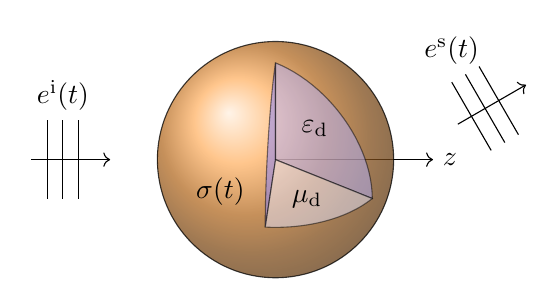
\begin{tikzpicture}

    \def\R{1.5} % sphere radius
    \def\angEl{35} % elevation angle
    \def\angleLongitudeP{-110} % longitude of point P
    \def\angleLongitudeQ{-45} % longitude of point Q
    \def\angleLatitudeQ{30} % latitude  Q    ; 0 latitude of P 
    \def\angleLongitudeA{-20} % longitude of point A

    \draw[->] (0,0) -- (2,0) node[right]{$z$};
    \shade[ball color=orange!80,opacity=.75,draw=black] (0,0) circle (\R);
    \tdplotsetmaincoords{90+\angEl}{-5}
    \begin{scope}[tdplot_main_coords]
    \path (0,0,0) coordinate (O);
    \draw[fill=blue!50,opacity=0.5] plot[variable=\t,domain=0:90] (xyz spherical cs:radius=\R,longitude=0,latitude=\t) -- (O) -- cycle;
    \draw[fill=blue!30,opacity=0.5] plot[variable=\t,domain=0:90] (xyz spherical cs:radius=\R,longitude=60,latitude=\t) -- (O) -- cycle;
    \draw[fill=blue!10,opacity=0.5] plot[variable=\t,domain=0:60] (xyz spherical cs:radius=\R,longitude=\t,latitude=0) -- (O) -- cycle;
    \end{scope}
    
    \node at (0.5,0.4) {$\varepsilon_\T{d}$};
        \node at (0.4,-0.5) {$\mu_\T{d}$};
    \node at (-0.7,-0.4) {$\sigma(t)$};
    
    \draw (-2.5,-0.5) -- (-2.5,0.5);
    \draw (-2.7,-0.5) -- (-2.7,0.5) node[above] {$e^\T{i}(t)$};
    \draw (-2.9,-0.5) -- (-2.9,0.5);
    \draw[->] (-3.1,0)--(-2.1,0);
    
    \begin{scope}[shift={(5,2)},rotate=30]
        \draw (-2.5,-0.5) -- (-2.5,0.5);
        \draw (-2.7,-0.5) -- (-2.7,0.5) node[above] {$e^\T{s}(t)$~~~~};
        \draw (-2.9,-0.5) -- (-2.9,0.5);
        \draw[->] (-3.1,0)--(-2.1,0);
    \end{scope}

    \end{tikzpicture}    
    \caption{A sphere of radius $a$ contains a static, non-dispersive material with permittivity and permeability $\varepsilon_\T{d} = \varepsilon_\T{r}\varepsilon_0$ and $\mu_\T{d} = \mu_\T{r}\mu_0$, respectively.  The surface of the sphere is coated with a time-varying surface conductivity $\sigma(t)$.}
    \label{fig:schem}
\end{figure}

We begin by considering a situation where the sphere is illuminated by a multi-frequency incident plane wave $\V{e}_\T{i}(t)$ and $\V{h}_\T{i}(t)$ with Fourier components of the form
\begin{equation}
    \V{E}^\T{i}(\omega) = \u{x}E(\omega)\T{e}^{-\T{j}kz},\quad
    \V{H}^\T{i}(\omega) = \u{y}\eta^{-1}E(\omega)\T{e}^{-\T{j}kz},
\end{equation}
where $k$ is the free space wavenumber at frequency $\omega$ and $\eta$ is the free space wave impedance.  At each frequency this wave may be expanded into spherical harmonics, leading to the tangential field components \cite[\S 7.4.3]{jin2011theory}
\begin{multline} \label{eq:pwexp-et}
    E_\theta^\T{i}(\omega) = - \frac{E_0 g(\omega)\cos\phi}{kr}\sum_{n=1}^{\infty} \T{j}^{-n}\frac{2n+1}{n(n+1)}\\\times\biggl[\T{j}\Jh'_n(kr)\frac{\T{d}\T{P}_n^1(\cos\theta)}{\T{d}\theta}+\Jh_n(kr)\frac{\T{P}_n^1(\cos\theta)}{\sin\theta}\biggr]
\end{multline}
\begin{multline}
    E_\phi^\T{i}(\omega) = \frac{E_0 g(\omega)\sin\phi}{kr}\sum_{n=1}^{\infty} \T{j}^{-n}\frac{2n+1}{n(n+1)}\\\times\left[\T{j}\Jh'_n(kr)\frac{\T{P}_n^1(\cos\theta)}{\sin\theta}+\Jh_n(kr)\frac{\T{d}\T{P}_n^1(\cos\theta)}{\T{d}\theta}\right]
\end{multline}
\begin{multline}
    H_\theta^\T{i}(\omega) = - \frac{E_0 g(\omega)\sin\phi}{\eta kr}\sum_{n=1}^{\infty} \T{j}^{-n}\frac{2n+1}{n(n+1)}\\\times\left[\Jh_n(kr)\frac{\T{P}_n^1(\cos\theta)}{\sin\theta}+\T{j}\Jh'_n(kr)\frac{\T{d}\T{P}_n^1(\cos\theta)}{\T{d}\theta}\right]
\end{multline}
\begin{multline}\label{eq:pwexp-hp}
    H_\phi^\T{i}(\omega) = - \frac{E_0 g(\omega)\cos\phi}{\eta kr}\sum_{n=1}^{\infty} \T{j}^{-n}\frac{2n+1}{n(n+1)}\\\times\left[\Jh_n(kr)\frac{\T{d}\T{P}_n^1(\cos\theta)}{\T{d}\theta}+\T{j}\Jh'_n(kr)\frac{\T{P}_n^1(\cos\theta)}{\sin\theta}\right]
\end{multline}
where $\Jh_n$ are spherical Riccati-Bessel functions and $\T{P}_n^1$ are associated Legendre polynomials.  Here $E_0$ represents a reference field magnitude while the unitless factor $g(\omega)$ indicates spectral weighting.

\begin{figure*}
\setcounter{tempEQCounter}{\value{equation}}
\setcounter{equation}{24}
\begin{multline}
    g_n =  \T{j}^{-1}\mu_\T{r}^{-1}\sqrt{\varepsilon_\T{r}}^{-1}\left[\sqrt{\mu_\T{r}}\Hh_n(ka)\Jh_n'(k_\T{d}a) -\sqrt{\varepsilon_\T{r}}\Hhp_n(ka)\Jh_n(k_\T{d}a)\right]c_n \\+ \omega\sqrt{\varepsilon_\T{r}\mu_\T{r}}^{-1}\Hhp_n(ka)\int_{-\infty}^\infty \omega^{\circ-1} \eta\hat{\sigma}(\omega-\omega^\circ)c_n(\omega^\circ)\Jh_n'(k^\circ_\T{d}a) \T{d}\omega^\circ.
    \label{eq:g-c-tm-long}
\end{multline}
\setcounter{equation}{\value{tempEQCounter}}
\hrulefill
\vspace*{4pt}
\end{figure*}

We may also expand the unknown scattered and internal fields at each frequency into similar spherical harmonics, matching the form of terms in the spherical wave expansion of the incident plane wave.  For the scattered field, this expansion reads
\begin{multline}
    E_\theta^\T{s}(\omega) = -\frac{E_0\cos\phi}{kr}\sum_{n=1}^\infty\\\left[a_n\T{j}\Hhp_n(kr)\frac{\T{d}\T{P}_n^1(\cos\theta)}{\T{d}\theta}+b_n\Hh_n(kr)\frac{\T{P}_n^1(\cos\theta)}{\sin\theta}\right]
    \label{eq:E-sc-t}
\end{multline}
\begin{multline}
    E_\phi^\T{s}(\omega) = \frac{E_0\sin\phi}{kr}\sum_{n=1}^\infty\\\left[a_n\T{j}\Hhp_n(kr)\frac{\T{P}_n^1(\cos\theta)}{\sin\theta}+b_n\Hh_n(kr)\frac{\T{d}\T{P}_n^1(\cos\theta)}{\T{d}\theta}\right]
    \label{eq:E-sc-p}
\end{multline}
\begin{multline}
    H_\theta^\T{s}(\omega) = -\frac{E_0\sin\phi}{\eta kr}\sum_{n=1}^\infty\\\left[a_n\Hh_n(kr)\frac{\T{P}_n^1(\cos\theta)}{\sin\theta}+b_n\T{j}\Hhp_n(kr)\frac{\T{d}\T{P}_n^1(\cos\theta)}{\T{d}\theta}\right]
    \label{eq:H-sc-t}
\end{multline}
\begin{multline}
    H_\phi^\T{s}(\omega) = -\frac{E_0\cos\phi}{\eta kr}\sum_{n=1}^\infty\\\left[a_n\Hh_n(kr)\frac{\T{d}\T{P}_n^1(\cos\theta)}{\T{d}\theta}+b_n\T{j}\Hhp_n(kr)\frac{\T{P}_n^1(\cos\theta)}{\sin\theta}\right]
    \label{eq:H-sc-p}
\end{multline}
and for the internal field we have
\begin{multline}
    E_\theta^\T{d}(\omega) =  -\frac{E_0\cos\phi}{k_\T{d}r}\sum_{n=1}^\infty\\\left[c_n\T{j}\Jh_n'(k_\T{d}r)\frac{\T{d}\T{P}_n^1(\cos\theta)}{\T{d}\theta}+d_n\Jh_n(k_\T{d}r)\frac{\T{P}_n^1(\cos\theta)}{\sin\theta}\right]
\end{multline}
\begin{multline}
    E_\phi^\T{d}(\omega) = \frac{E_0\sin\phi}{k_\T{d}r}\sum_{n=1}^\infty\\\left[c_n\T{j}\Jh_n'(k_\T{d}r)\frac{\T{P}_n^1(\cos\theta)}{\sin\theta}+d_n\Jh_n(k_\T{d}r)\frac{\T{d}\T{P}_n^1(\cos\theta)}{\T{d}\theta}\right]
\end{multline}
\begin{multline}
    H_\theta^\T{d}(\omega) = -\frac{E_0\sin\phi}{\eta_\T{d}k_\T{d}r}\sum_{n=1}^\infty\\\left[c_n\Jh_n(k_\T{d}r)\frac{\T{P}^1_n(\cos\theta)}{\sin\theta} + d_n\T{j}\Jh_n'(k_\T{d}r)\frac{\T{d}\T{P}_n^1(\cos\theta)}{\T{d}\theta}\right]
\end{multline}
\begin{multline}
    H_\phi^\T{d}(\omega) =  -\frac{E_0\cos\phi}{\eta_\T{d}k_\T{d}r}\sum_{n=1}^\infty\\\left[c_n\Jh_n(k_\T{d}r)\frac{\T{d}\T{P}_n^1(\cos\theta)}{\T{d}\theta} + d_n\T{j}\Jh_n'(k_\T{d}r)\frac{\T{P}^1_n(\cos\theta)}{\sin\theta}\right].
\end{multline}
In the above expressions, $k_\T{d}$ and $\eta_\T{d}$ denote the wavenumber and characteristic impedance of the core material, respectively.  The coefficients $\{a_n\}$ and $\{c_n\}$ are associated with transverse magnetic (TM) modes, while $\{b_n\}$ and $\{d_n\}$ correspond to transverse electric (TE) modes. 

Tangential field continuity at the boundary of the sphere gives rise to four boundary conditions that must hold for all times $t$, specifically
\begin{equation}
    e_\theta^\T{i}(t)+e_\theta^\T{s}(t)=
    e_\theta^\T{d}(t)
    \label{eq:e-theta-cont}
\end{equation}
\begin{equation}
    e_\phi^\T{i}(t)+e_\phi^\T{s}(t) = 
    e_\phi^\T{d} (t)
    \label{eq:e-phi-cont}
\end{equation}
\begin{equation}
    h_\theta^\T{i}(t)+h_\theta^\T{s}(t) = 
    h_\theta^\T{d}(t) + \sigma(t)e_\phi^\T{d}(t)
    \label{eq:h-theta-cont}
\end{equation}
\begin{equation}
    h_\phi^\T{i}(t)+h_\phi^\T{s}(t) = 
    h_\phi^\T{d}(t) - \sigma(t)e_\theta^\T{d}(t).
    \label{eq:h-phi-cont}
\end{equation}
Within the magnetic field boundary conditions \eqref{eq:h-theta-cont} and \eqref{eq:h-phi-cont}, terms of the form $\sigma(t)e_{x}^\T{d}(t)$ represent a surface current density. % clarifying the units of of the surface conductivity $\sigma(t)$ as $\Omega^{-1}$. 
Temporal phase matching gives analogous conditions on each Fourier component of the fields.  Applying the series forms of incident, internal, and scattered fields in the frequency domain and matching terms of like tangential dependence, the first pair of boundary conditions \eqref{eq:e-theta-cont} and \eqref{eq:e-phi-cont} gives
\begin{equation}
    g_n\Jh'_n(ka) + a_n\Hhp_n(ka) = \frac{k}{k_\T{d}}c_n\Jh_n'(k_\T{d}a)
    \label{eq:bc-e-tm}
\end{equation}
\begin{equation}
    g_n\Jh_n(ka) + b_n\Hh_n(ka) =\frac{k}{k_\T{d}}d_n\Jh_n(k_\T{d}a)
\end{equation}
where 
\begin{equation}
    g_n = g(\omega)\T{j}^{-n}\frac{2n+1}{n(n+1)}
\end{equation}
and the frequency dependence of $g_n$, $a_n$, $b_n$, $c_n$, and $d_n$ has been suppressed.  Since multiplication in the time domain results in convolution in the frequency domain, the second set of boundary conditions in \eqref{eq:h-theta-cont} and \eqref{eq:h-phi-cont} is more complex, reading 
\begin{multline}
    g_n\Jh_n(ka)+a_n\Hh_n(ka) = \frac{\mu}{\mu_\T{d}}c_n \Jh_n(k_\T{d}a) \\- \T{j} k\eta\int_{-\infty}^\infty k_\T{d}^{\circ-1} \hat{\sigma}(\omega-\omega^\circ)c_n(\omega^\circ)\Jh_n'(k^\circ_\T{d}a) \T{d}\omega^\circ,
    \label{eq:bc-h-tm}
\end{multline}
\begin{multline}
    g_n\Jh_n'(ka)+b_n\Hhp_n(ka) = \frac{\mu}{\mu_\T{d}}d_n \Jh_n'(k_\T{d}a) \\+ \T{j} k\eta\int_{-\infty}^\infty k_\T{d}^{\circ-1} \hat{\sigma}(\omega-\omega^\circ)d_n(\omega^\circ)\Jh_n(k^\circ_\T{d}a) \T{d}\omega^\circ.
\end{multline}
Here $^\circ$ is used to mark integration variables as $'$ is already used to denote differentiation of a function with respect to its argument.  Considering the functions $g_n$, $a_n$, $b_n$, $c_n$, and $d_n$ described by a basis of monochromatic signals, we may interpret all terms in the above boundary conditions as diagonal operators, with the exception of the convolution terms which naturally give rise to cross frequency coupling.  As expected, we see that the TE and TM excitation coefficients are fully decoupled.  



We first consider the system of equations governing the TM coefficients.  Solving \eqref{eq:bc-e-tm} for the external coefficients $a_n$ gives
\begin{equation}
     a_n = \frac{1}{\Hhp_n(ka)}\left[\frac{k}{k_\T{d}}c_n\Jh_n'(k_\T{d}a) - g_n\Jh_n'(ka)\right].
    \label{eq:an-cn}
\end{equation}
Using this expression to eliminate the external coefficients from \eqref{eq:bc-h-tm} and collecting terms leads to \eqref{eq:g-c-tm-long}\stepcounter{equation}, where the Riccati-Bessel function Wronskian identity~\cite{abramowitz1948handbook}
\begin{equation}
    \Jh_n(z)\Hhp_n(z) - \Jh_n'(z)\Hh_n(z) = -\T{j}
    \label{eq:h2-wronsk}
\end{equation}
has been used.  Defining the operators
\begin{multline}
    \mathcal{A}_n x = \T{j}^{-1}\mu_\T{r}^{-1}\sqrt{\varepsilon_\T{r}}^{-1}\\\times\left[\sqrt{\mu_\T{r}}\Hh_n(ka)\Jh_n'(k_\T{d}a) -\sqrt{\varepsilon_\T{r}}\Hhp_n(ka)\Jh_n(k_\T{d}a)\right]x
\end{multline}
and
\begin{multline}
    \mathcal{B}_n x = \omega\sqrt{\varepsilon_\T{r}\mu_\T{r}}^{-1}\Hhp_n(ka)\\\times\int_{-\infty}^\infty \omega^{\circ-1}\eta\hat{\sigma}(\omega-\omega^\circ)x(\omega^\circ)\Jh_n'(k^\circ_\T{d}a) \T{d}\omega^\circ
\end{multline}
allows for a condensed form of \eqref{eq:g-c-tm-long} to be written as
\begin{equation}
    g_n = \left(\mathcal{A}_n+\mathcal{B}_n\right)c_n.
    \label{eq:gn-tm-cont}
\end{equation}
Again, with respect to a basis of monochromatic signals, the operator $\mathcal{A}_n$ is always diagonal, whereas the operator $\mathcal{B}_n$ associated with the surface conductivity is, in general, not diagonal.  From this reduced operator expression, we immediately recognize simplifications arising from several important special cases.  First, when the surface conductivity is identically zero the operator $\mathcal{B}_n$ vanishes, yielding the classical TM scattering coefficients for a dielectric sphere.  Similarly, if the surface conductivity is purely static (not varying in time) the operator $\mathcal{B}_n$ becomes diagonal~\cite{wait1965calculations}. Additionally, if the inner medium has the same material properties as the external medium (i.e., $\varepsilon_\T{r} = \mu_\T{r} = 1$), then $\mathcal{A}_n$ becomes the identity operator.  Two special cases reduce the above system to one of a PEC sphere, either $\sigma(t)\rightarrow\infty$ for all time or  $\varepsilon_\T{r}\rightarrow -\T{j}\infty$.  



Repeating the above analysis for TE modes we find the external coefficients to be
\begin{equation}
    b_n = \frac{1}{\Hh_n(ka)}\left[\frac{k}{k_\T{d}}d_n\Jh_n(k_\T{d}a) - g_n\Jh_n(ka)\right]
    \label{eq:bn-dn}
\end{equation}
and the internal coefficients given by
\begin{equation}
    g_n = (\mathcal{C}_n + \mathcal{D}_n)d_n
    \label{eq:gn-te-cont}
\end{equation}
where
\begin{multline}
    \mathcal{C}_n x = \T{j}^{-1}\mu_\T{r}^{-1}\sqrt{\varepsilon_\T{r}}^{-1}\\\times\left[\sqrt{\varepsilon_\T{r}}\Hh_n(ka)\Jh_n'(k_\T{d}a) -\sqrt{\mu_\T{r}}\Hhp_n(ka)\Jh_n(k_\T{d}a)\right]x
    \label{eq:cnx}
\end{multline}
and
\begin{multline}
    \mathcal{D}_n x = \omega\sqrt{\varepsilon_\T{r}\mu_\T{r}}^{-1}\Hh_n(ka)\\\times\int_{-\infty}^\infty \omega^{\circ-1}\eta\hat{\sigma}(\omega-\omega^\circ)x(\omega^\circ)\Jh_n(k^\circ_\T{d}a) \T{d}\omega^\circ.
\end{multline}


\begin{figure*}
\setcounter{tempEQCounter}{\value{equation}}
\setcounter{equation}{41}
\begin{multline}
    \M{B}_n = \eta \sqrt{\varepsilon_\T{r}\mu_\T{r}}^{-1} 
    \begin{bmatrix}
    \omega_{-K}\Hhp_n(k^{-K}a) & 0 & 0 & 0 \\
    0 & \omega_{-K+1}\Hhp_n(k^{-K+1}a) & 0 & 0\\
    0 & 0 & \ddots & 0\\
    0 & 0 & 0 & \omega_{K}\Hhp_n(k^{K}a)
    \end{bmatrix}\\
\begin{bmatrix}
    \hat{\sigma}^{0} &  \hat{\sigma}^{-1} & \hdots & \hat{\sigma}^{-2K} \\
    \hat{\sigma}^{1} &  \hat{\sigma}^0 & \hdots & \hat{\sigma}^{-2K+1} \\
    \vdots & \vdots & \vdots & \vdots\\
    \hat{\sigma}^{2K} &  \hat{\sigma}^{2K-1} & \hdots & \hat{\sigma}^0 \\
    \end{bmatrix}
    \begin{bmatrix}
    \omega^{-1}_{-K}\Jh_n'(k^{-K}_\T{d}a) & 0 & 0 & 0 \\
    0 & \omega_{-K+1}^{-1}\Jh_n'(k^{-K+1}_\T{d}a) & 0 & 0\\
    0 & 0 & \ddots & 0\\
    0 & 0 & 0 & \omega_{K}^{-1}\Jh_n'(k^{K}_\T{d}a)
    \end{bmatrix}
    \label{eq:bmatrix-long}
\end{multline}
\setcounter{equation}{\value{tempEQCounter}}
\end{figure*}

\begin{figure*}
\setcounter{tempEQCounter}{\value{equation}}
\setcounter{equation}{44}
\begin{multline}
    \M{D}_n = \eta \sqrt{\varepsilon_\T{r}\mu_\T{r}}^{-1} 
    \begin{bmatrix}
    \omega_{-K}\Hh_n(\omega_{-K} a/c) & 0 & 0 & 0 \\
    0 & \omega_{-K+1}\Hh_n(\omega_{-K+1} a/c) & 0 & 0\\
    0 & 0 & \ddots & 0\\
    0 & 0 & 0 & \omega_{K}\Hh_n(\omega_{K} a/c)
    \end{bmatrix}\\
\begin{bmatrix}
    \hat{\sigma}^{0} &  \hat{\sigma}^{-1} & \hdots & \hat{\sigma}^{-2K} \\
    \hat{\sigma}^{1} &  \hat{\sigma}^0 & \hdots & \hat{\sigma}^{-2K+1} \\
    \vdots & \vdots & \vdots & \vdots\\
    \hat{\sigma}^{2K} &  \hat{\sigma}^{2K-1} & \hdots & \hat{\sigma}^0 \\
    \end{bmatrix}
    \begin{bmatrix}
    \omega_{-K}^{-1}\Jh_n(k^{-K}_\T{d}a) & 0 & 0 & 0 \\
    0 & \omega_{-K+1}^{-1}\Jh_n(k^{-K+1}_\T{d}a) & 0 & 0\\
    0 & 0 & \ddots & 0\\
    0 & 0 & 0 & \omega_{K}^{-1}\Jh_n(k^{K}_\T{d}a)
    \end{bmatrix}
    \label{eq:dmatrix-long}
\end{multline}
\hrulefill
\vspace*{4pt}
\end{figure*}
\setcounter{equation}{\value{tempEQCounter}}


\section{Fourier series expansion of surface parameters}
\label{sec:fourier}

The preceding formulation involves integral operators whose kernels depend on the frequency domain representation of the surface conductivity $\hat{\sigma}(\omega)$.  In order to systematically solve these equations, we consider the special case in which the time-variation of the surface conductivity is periodic.  The aim of this simplification is to recast \eqref{eq:gn-tm-cont} and \eqref{eq:gn-te-cont} as matrix equations, similar to the construction of conversion matrices in time-varying circuit analysis \cite{maas2003nonlinear}.

Let the surface conductivity be expressible in terms of a Fourier series with fundamental frequency $\omega_\sigma$, i.e.,
\begin{equation}
    \hat{\sigma}(\omega) = \sum_{q=-K}^{K}\hat{\sigma}^q\delta(\omega-q\omega_\sigma).
\end{equation}
Substitution into the operator $\mathcal{B}_n$ gives, via the sifting property of the Dirac delta,
\begin{multline}
    \mathcal{B}_n x = \omega\eta\sqrt{\varepsilon_\T{r}\mu_\T{r}}^{-1}\Hhp_n(\omega a/c)\\\times\sum_{q=-K}^{K}\hat{\sigma}^q (\omega-q\omega_\sigma)^{-1}\Jh_n'((\omega-q\omega_\sigma)a/c_\T{d}) x(\omega-q\omega_\sigma),
\end{multline}
where $c$ and $c_\T{d}$ are the speed of light in vacuum and the dielectric core, respectively.  Further, assume that the excitation has a center frequency $\omega_0$ and a baseband representation that is periodic in the fundamental frequency $\omega_\sigma$, i.e.,
\begin{equation}
    g_n(\omega) = \sum_{p = -K}^K g_n^p\delta(\omega-\omega_0-p\omega_\sigma).
\end{equation}
Using these assumptions, \eqref{eq:gn-tm-cont} evaluated at frequency $\omega_p = \omega_0 + p\omega_\sigma$ may be written,
\begin{equation}
    g_n^p = A_n^{p}c_n^p +\sum_{q=-K}^K B_n^{pq}c_n^{p-q},
\end{equation}
with $c_n^p = c_n(\omega_p)$,
\begin{multline}
    A_n^{p} = \T{j}^{-1}\mu_\T{r}^{-1}\sqrt{\varepsilon_\T{r}}^{-1}\biggl[\sqrt{\mu_\T{r}}\Hh_n(k^p a)\Jh_n'(k^p_\T{d}a) \\ -\sqrt{\varepsilon_\T{r}}\Hhp_n(k^p a)\Jh_n(k^p_\T{d}a)\biggr],
    \label{eq:anp}
\end{multline}
and
\begin{multline}
    B_n^{pq} =  \omega_p\eta\sqrt{\varepsilon_\T{r}\mu_\T{r}}^{-1} \Hhp_n(k^p a)\hat{\sigma}^q\Jh_n'(k^{p-q}_\T{d}a)\omega_{p-q}^{-1}
    \label{eq:bnpq}
\end{multline}
where $k^p$ and $k^p_\T{d}$ are the wavenumbers at frequency $\omega_p$ in the exterior and core materials, respectively.  A set of $2K+1$ equations of this form may be collected into the system 
\begin{equation}
    \M{g}_n = \left(\M{A}_n + \M{B}_n\right)\M{c}_n
    \label{eq:g-vector-tm}
\end{equation}
where
\begin{equation}
    \M{A}_n = \begin{bmatrix}
    A_n^{-K} & 0 & 0 & 0 \\
    0 & A_n^{-K+1} & 0 & 0\\
    0 & 0 & \ddots & 0\\
    0 & 0 & 0 & A_n^K
    \end{bmatrix}
\end{equation}
and the matrix $\M{B}_n$ is given in factored form in \eqref{eq:bmatrix-long}.  This factorization is most easily constructed from \eqref{eq:bnpq} by substituting $\beta = p-q$ and inspecting the elements $B_n^{p\beta}$.

\setcounter{equation}{42}
Similarly for the TE coefficients we may write
\begin{equation}
    \M{g}_n = \left(\M{C}_n + \M{D}_n\right)\M{d}_n
    \label{eq:g-vector-te}
\end{equation}
where
\begin{equation}
    \M{C}_n = \begin{bmatrix}
    C_n^{-K} & 0 & 0 & 0 \\
    0 & C_n^{-K+1} & 0 & 0\\
    0 & 0 & \ddots & 0\\
    0 & 0 & 0 & C_n^K
    \end{bmatrix}
\end{equation}
\setcounter{equation}{44}
with elements analogous to \eqref{eq:anp} based on \eqref{eq:cnx} and the matrix $\M{D}_n$ as given in \eqref{eq:dmatrix-long}\stepcounter{equation}.  The form of the inner matrix
\begin{equation}
    \bs{\sigma} = \begin{bmatrix}
    \hat{\sigma}^{0} &  \hat{\sigma}^{-1} & \hdots & \hat{\sigma}^{-2K} \\
    \hat{\sigma}^{1} &  \hat{\sigma}^0 & \hdots & \hat{\sigma}^{-2K+1} \\
    \vdots & \vdots & \vdots & \vdots\\
    \hat{\sigma}^{2K} &  \hat{\sigma}^{2K-1} & \hdots & \hat{\sigma}^0 \\
    \end{bmatrix}
\end{equation}
closely resembles that of the conversion matrix describing multi-harmonic coupling in time-varying circuit analysis \cite{maas2003nonlinear} or method of moments problems involving time-varying loads and materials \cite{bass2021conversion}.  Interpretation of this quantity as the conversion matrix representation of a time-varying admittance is discussed further in Sec.~\ref{sec:tl}.

Together \eqref{eq:g-vector-tm} and \eqref{eq:g-vector-te} allow for the calculation of the internal Fourier components $\M{c}_n$ and $\M{d}_n$, from which the external terms $\M{a}_n$ and $\M{b}_n$ are obtained via \eqref{eq:an-cn} and \eqref{eq:bn-dn}, respectively.  Adopting the alternative modal normalization of Bohren and Huffman~\cite{bohren2008absorption}, we define new sets of external coefficients
\begin{equation}
    \tilde{\M{a}}_n = -\M{a}_n\frac{n(n+1)}{\T{j}^{-n}(2n+1)},\quad \tilde{\M{b}}_n = -\M{b}_n\frac{n(n+1)}{\T{j}^{-n}(2n+1)}.
\end{equation}
Assuming a monochromatic incident wave of power density $S_0$ at frequency $\omega_0$, this renormalization leads to a familiar form for the normalized net scattered power (scattering efficiency) at each frequency,
\begin{equation}
    Q_\T{sc}^p = \frac{P_\T{sc}^p}{S_0 \pi a^2} = \frac{2c^2}{\omega_p^2a^2}\sum_{n=1}^\infty (2n+1)\left[|\tilde{a}_n^p|^2 + |\tilde{b}_n^p|^2\right].
\end{equation}
The normalized extinction power (extinction efficiency) takes on a similar form
\begin{equation}
    Q_\T{ext}^0 = \frac{P_\T{ext}^0}{S_0 \pi a^2} = \frac{2c^2}{\omega_0^2a^2}\sum_{n=1}^\infty (2n+1)\T{Re}\,\left\{\tilde{a}_n^0 + \tilde{b}_n^0\right\}.
\end{equation}
By assuming monochromatic incidence, the extinction efficiency is only defined for the $p=0$ harmonic.  Because the time-varying scattering processes considered here are linear\footnote{See \cite[\S 3.4.1]{maas2003nonlinear} for extended discussion of conversion matrix linearity in the context of circuit problems.}, extended definitions of polychromatic scattering and extinction efficiencies may be constructed similarly to those used to describe polarization conversion processes in scattering cross section analyses.

\section{Surface resistance and conductivity}

The time-variation of the surface conductivity $\sigma(t)$ may be alternatively described using surface resistance $r(t) = \sigma(t)^{-1}$.  Note that simple time-variations in one parameter may be problematic or ill-defined in terms of the other.  For example, the simple time-varying surface resistance
\begin{equation}
    r(t) = r_0\left(1+\gamma\cos \omega_\sigma t\right),\quad \gamma\leq 1
    \label{eq:r-single-harm}
\end{equation}
has a well-behaved Fourier spectrum, however the associated surface conductivity tends toward a train of Dirac delta functions as $\gamma \rightarrow 1$ and $r_0\rightarrow \infty$.  This, in turn, necessitates the use of extreme numbers of frequencies in the solution of scattered fields which may lead to non-convergent results.  Throughout this paper we consider examples using conductance and resistance of the above form to examine this behavior.


\newcommand{\upia}{\V{u}_\alpha^{(1)}}
\newcommand{\upiab}{\V{u}_{\bar{\alpha}}^{(1)}}
\newcommand{\uppa}{\V{u}_\alpha^{(\rbkind)}}
\newcommand{\uppab}{\V{u}_{\bar{\alpha}}^{(\rbkind)}}
\newcommand{\upoa}{\V{u}_\alpha^{(4)}}
\newcommand{\upoab}{\V{u}_{\bar{\alpha}}^{(4)}}
\newcommand{\Ra}{\T{R}_\alpha}
\newcommand{\Rb}{\T{R}_{\bar{\alpha}}}


\section{Transition matrix formulation}
\label{sec:tmat}
\begin{figure*}
\setcounter{tempEQCounter}{\value{equation}}
\setcounter{equation}{66}
\begin{multline}
    \Ymat_\alpha = -\T{j}\eta \gamma_\alpha 
    \begin{bmatrix}
    W_\alpha^{-K} & 0 & 0 & 0 \\
    0 & W_\alpha^{-K+1} & 0 & 0\\
    0 & 0 & \ddots & 0\\
    0 & 0 & 0 & W_\alpha^{K}
    \end{bmatrix}^{-1}
    \begin{bmatrix}
    \Ra^{(4)}(k^{-K}a) & 0 & 0 & 0 \\
    0 & \Ra^{(4)}(k^{-K+1}a) & 0 & 0\\
    0 & 0 & \ddots & 0\\
    0 & 0 & 0 & \Ra^{(4)}(k^{K} a)
    \end{bmatrix}\\
    \begin{bmatrix}
    \hat{\sigma}^{0} &  \hat{\sigma}^{-1} & \hdots & \hat{\sigma}^{-2K} \\
    \hat{\sigma}^{1} &  \hat{\sigma}^0 & \hdots & \hat{\sigma}^{-2K+1} \\
    \vdots & \vdots & \vdots & \vdots\\
    \hat{\sigma}^{2K} &  \hat{\sigma}^{2K-1} & \hdots & \hat{\sigma}^0 \\
    \end{bmatrix}
    \begin{bmatrix}
    \Ra^{(1)}(k_\T{d}^{-K}a) & 0 & 0 & 0 \\
    0 & \Ra^{(1)}(k_\T{d}^{-K+1}a) & 0 & 0\\
    0 & 0 & \ddots & 0\\
    0 & 0 & 0 & \Ra^{(1)}(k_\T{d}^{K}a)
    \end{bmatrix}
    \label{eq:ymatrix-long}
\end{multline}
\hrulefill
\vspace*{4pt}
\end{figure*}
\setcounter{equation}{\value{tempEQCounter}}

In preceding sections we explicitly considered incident fields of the form of plane waves.  The formulation may be extended to more general illuminations through the use of transition (T-) matrix formalism \cite{waterman1965matrix,chew1990inhomogeneous}.  Consider an incident field of the form
\begin{equation}\label{eq:einc}
    \V{E}^\T{i}(\omega,\V{r}) = \sum_\alpha \upia(k\V{r}) g_\alpha
\end{equation}
where $\upia$ are vector spherical harmonics~\cite{ScatteringofEMWavesbyObstacles} associated with Riccati-Bessel functions of the first kind, see App.~\ref{sec:special-functions}.  By the addition theorem for vector spherical waves, this expansion is capable of representing any incident field produced by sources at locations $\V{r}'$ outside of the region of interest, i.e., $r<r'$~\cite[Eq. 7.5.14]{jin2011theory}. In a similar manner, the scattered and internal fields may be expanded as
\begin{equation}\label{eq:escat}
    \V{E}^\T{s}(\omega,\V{r}) = \sum_\alpha \upoa(k\V{r}) f_\alpha
\end{equation}
\begin{equation}\label{eq:ediel}
    \V{E}^\T{d}(\omega,\V{r}) = \sum_\alpha \upia(k_\T{d}\V{r}) h_\alpha
\end{equation}
where $\upoa$ are vector spherical harmonics associated with Riccati-Hankel functions of the second kind.  The property \cite[Eq. 7.2.4]{chew1990inhomogeneous}
\begin{equation}
    \nabla\times\uppa = k\uppab
\end{equation}
relates two classes of spherical vector waves with dual superindices $\alpha$ and $\bar{\alpha}$ \cite{losenicky2020method}.  By virtue of this property, the magnetic fields associated with incident, scattered, and internal electric fields are given by 
\begin{equation}\label{eq:hinc}
    \V{H}^\T{i}(\omega,\V{r}) = \T{j}\eta^{-1}\sum_\alpha \upiab(k\V{r}) g_\alpha
\end{equation}
\begin{equation}\label{eq:hscat}
    \V{H}^\T{s}(\omega,\V{r}) = \T{j}\eta^{-1}\sum_\alpha \upoab(k\V{r}) f_\alpha
\end{equation}
\begin{equation}\label{eq:hdiel}
    \V{H}^\T{d}(\omega,\V{r}) = \T{j}\eta_\T{d}^{-1}\sum_\alpha \upiab(k_\T{d}\V{r}) h_\alpha.
\end{equation}

Tangential electric field continuity in \eqref{eq:e-theta-cont} and \eqref{eq:e-phi-cont} at the sphere's boundary leads to
\begin{equation}
    g_\alpha\Ra^{(1)}(ka) + f_\alpha \Ra^{(4)}(ka) = h_\alpha \Ra^{(1)}(k_\T{d}a),
    \label{eq:tmat-e-cont}
\end{equation}
where $\Ra^{(p)}$ describe the radial dependence of spherical waves $\uppa$, see App.~\ref{sec:special-functions}.  Similarly, the magnetic field boundary conditions in \eqref{eq:h-theta-cont} and \eqref{eq:h-phi-cont} lead to 
\begin{multline}
    g_\alpha \Rb^{(1)}(ka) + f_\alpha\Rb^{(4)}(ka) = \frac{\eta}{\eta_\T{d}}h_\alpha \Rb^{(1)}(k_\T{d}a) \\- \T{j}\eta\gamma_\alpha\hat{\sigma}\star\left[h_\alpha\Ra^{(1)}(k_\T{d}a)\right]
    \label{eq:tmat-h-cont}
\end{multline}
where the identity
\begin{equation}\label{eq:signconstdefn}
    \u{r}\times\left(\u{r}\times\V{u}^{(\rbkind)}_{\bar\alpha}(\u{r})\right) = \u{r}\times\gamma_\alpha\V{u}^{(\rbkind)}_{\alpha}(\u{r}),\quad \gamma_\alpha = -1^{\tau}
\end{equation}
has been employed to relate tangential field components of harmonics with dual superindices. Note that the index $\tau$ is contained within the superindex $\alpha$, see Appendix A. 
Eliminating the external coefficients $f_\alpha$ gives 
\begin{equation}
    g_\alpha = (\Xop_\alpha+\Yop_\alpha)h_\alpha
    \label{eq:tmat-op-eq}
\end{equation}
where the operators $\Xop_\alpha$ and $\Yop_\alpha$ have the forms
\begin{multline}
    \Xop_\alpha x = \\\mathcal{W}_\alpha^{-1}\left[\frac{\eta}{\eta_\T{d}}\Ra^{(4)}(ka)\Rb^{(1)}(k_\T{d}a) - \Rb^{(4)}(ka)\Ra^{(1)}(k_\T{d}a)\right]x
    \label{eq:w-alpha}
\end{multline}
\begin{multline}
    \Yop_\alpha x = \\
    -\T{j}\eta \mathcal{W}_\alpha^{-1}\gamma_\alpha\Ra^{(4)}\int_{-\infty}^\infty \hat{\sigma}(\omega-\omega^\circ)x(\omega^\circ)\Ra^{(1)}(k^\circ_\T{d}a) \T{d}\omega^\circ
\end{multline}
with
\begin{equation}
    \mathcal{W}_\alpha x = \left[\Rb^{(1)}(ka)\Ra^{(4)}(ka) - \Ra^{(1)}(ka)\Rb^{(4)}(ka)\right]x.
    \label{eq:wdef}
\end{equation}
Adopting the Fourier series representations used in Sec.~\ref{sec:fourier}, we may convert the continuous operator equation in \eqref{eq:tmat-op-eq} into a matrix equation of the form
\begin{equation}
    \M{g}_\alpha = \left(\Xmat_\alpha + \Ymat_\alpha\right)\M{h}_\alpha
    \label{eq:tmat-mat-eq}
\end{equation}
where the matrix $\Xmat_\alpha$ is diagonal with elements
\begin{multline}
    \Xopchar_\alpha^{p} = W^{p,-1}_\alpha\\
    \times\left[\frac{\eta}{\eta_\T{d}}\Ra^{(4)}(k^pa)\Rb^{(1)}(k^p_\T{d}a) - \Rb^{(4)}(k^pa)\Ra^{(1)}(k^p_\T{d}a)\right]
\end{multline}
and the matrix $\Ymat_\alpha$ is given in factored form in \eqref{eq:ymatrix-long}\stepcounter{equation}.  Here the term $W^{p}_\alpha$ corresponds to the coefficient in \eqref{eq:wdef} evaluated at frequency $\omega_p$.  %We now eliminate the internal coefficients $\M{h}_\alpha$ in \eqref{eq:tmat-mat-eq} in favor of the external coefficients $\M{f}_\alpha$ using \eqref{eq:tmat-e-cont}.  
After some manipulations, this leads to a transition matrix system
\begin{equation}
    \M{f}_\alpha = \M{T}_\alpha\M{g}_\alpha
    \label{eq:tmat-def}
\end{equation}
where
\begin{equation}
    \M{T}_\alpha = \M{R}_{\alpha,4}^{-1}\left[\M{R}_{\alpha,1\T{d}}\left(\Xmat_\alpha+\Ymat_\alpha\right)^{-1}-\M{R}_{\alpha,1}\right]
    \label{eq:t-mat-final}
\end{equation}
with
\begin{equation}
    \M{R}_{\alpha,\rbkind} = \begin{bmatrix}
    \Ra^{(\rbkind)}(k^{-K}a) & 0 & 0 \\
    0  & \ddots & 0\\
    0  & 0 & \Ra^{(\rbkind)}(k^{K}a)
    \end{bmatrix}
    \label{eq:rp-mat}
\end{equation}
and    
\begin{equation}
    \M{R}_{\alpha,\rbkind\T{d}} = \begin{bmatrix}
    \Ra^{(\rbkind)}(k_\T{d}^{-K}a) & 0 & 0 \\
    0  & \ddots & 0\\
    0  & 0 & \Ra^{(\rbkind)}(k_\T{d}^{K}a)
    \end{bmatrix}.
    \label{eq:rpd-mat}
\end{equation}
The transition matrix in \eqref{eq:tmat-def} fully describes the scattering of multi-harmonic incident fields originating from sources exterior to the sphere under consideration.  Hence it is suitable, through proper application of the addition theorem, to adaptation toward the scattering analysis of collections of non-overlapping spherical structures. 


\section{Spherical waveguide perspective}
\label{sec:tl}
Here we consider an alternative transmission line perspective of the scattering problem presented in Secs.~\ref{sec:pw}, \ref{sec:fourier}, and~\ref{sec:tmat}. In general, we may consider the free space around the sphere as a spherical waveguide, in which each mode has an associated characteristic  admittance \cite{harrington2001time}. 
The wave admittance $Y_\alpha^{(\rbkind)}$ of a spherical wave defined by an electric field of the form $\V{u}_\alpha^{(\rbkind)}$ relates the magnitudes of the tangential electric and magnetic fields via
\begin{equation}
    \V{H}^{\T{tan}}_\alpha = Y^{(\rbkind)}_\alpha \u{r}\times\V{E}^{\T{tan}}_\alpha.
\end{equation}
Using \eqref{eq:einc} and \eqref{eq:hinc}, \eqref{eq:escat} and \eqref{eq:hscat}, or \eqref{eq:ediel} and \eqref{eq:hdiel} for the incident, scattered, or internal fields respectively, we define a diagonal multi-frequency wave admittance matrix
\begin{equation}
    \M{Y}_{\alpha,\rbkind m} = \T{j}\gamma_\alpha\eta_m^{-1}\M{R}_{\bar{\alpha}, \rbkind m} (\M{R}_{\alpha, \rbkind m})^{-1},
    \label{eq:admittance-mat}
\end{equation}
where, following the notation of \eqref{eq:rp-mat} and \eqref{eq:rpd-mat}, the subscript $\rbkind m$%of the diagonal Riccatti-Bessel function matrix
~may be either $\rbkind$ for waves of the $\rbkind$th kind in free space or $\rbkind\T{d}$ for waves in the dielectric core. Similarly, the impedance $\eta_m$ is either that of free space or the dielectric core. The sign constant $\gamma_\alpha$ is $\pm 1$ as given in \eqref{eq:signconstdefn}, which produces an appropriate sign for TE and TM modes.

The electric field continuity equation of \eqref{eq:tmat-e-cont} may be written in terms of incident, reflected, and transmitted ``voltages''%\footnote{These should be considered ``voltages'' in the general sense that the Method of Moments excitation vector contains ``voltages'' -- that is, inner products between the electric field and a set of basis functions, which in this case are the associated Legendre polynomials.} 
~at each frequency as 
\begin{equation}
    v^\T{i}_\alpha + v^\T{r}_\alpha = v^\T{t}_\alpha,
    \label{eq:tline-e-cont}
\end{equation}
where the incident voltages are
\begin{equation}
    v^\T{i}_\alpha = g_\alpha\Ra^{(1)}(ka),
\end{equation}
and similar forms are used for the reflected and transmitted terms.  Collecting equations of this kind at all frequencies we obtain the system of equations
\begin{equation}
    \M{v}_\alpha^\T{i} + \M{v}_\alpha^\T{r} = \M{v}^\T{t}_\alpha.
\end{equation}

Using the same voltage definitions along with admittance matrices of the form of \eqref{eq:admittance-mat}, the magnetic field  continuity equation of \eqref{eq:tmat-h-cont} may be written as
\begin{equation}\label{eq:TLcurrent2}
    \M{Y}_{\alpha,1} \M{v}^\T{i}_\alpha   + \M{Y}_{\alpha,4} \M{v}^\T{r}_\alpha  =  \M{Y}_{\alpha,1\T{d}}\M{v}^\T{t}_\alpha + \V{\sigma}\M{v^\T{t}}_\alpha,
\end{equation}
where the convolution term in \eqref{eq:tmat-h-cont} is represented by cross-frequency (off-diagonal) terms in the conversion matrix $\V{\sigma}$.

Interpreting \eqref{eq:tmat-e-cont} and \eqref{eq:TLcurrent2} as the voltage and current boundary conditions at a transmission line junction, it is clear that the surface of the sphere appears as a time-varying conductance in parallel with the input admittance ``looking into'' the core.  This configuration is depicted in Fig.~\ref{fig:TLschematic}, where a compressed notation is used to depict wave impedances in each region.  Because of the orthogonality of vector spherical harmonics, no mode conversion occurs at the surface of the sphere, but the time-varying boundary condition does result in frequency conversion. Thus, while each harmonic frequency satisfies \eqref{eq:tline-e-cont} independently, \eqref{eq:TLcurrent2} relates multiple harmonic frequencies simultaneously and cannot be separated into an independent equation for each frequency.

\begin{figure}
    \centering
        \begin{circuitikz}[
		%Environment Config
		%line width=0.75,
		%Style Variable
		text pos/.store in=\tpos,text pos=0.5,
		text anchor/.store in=\tanchor,text anchor={north:12pt},
		Tline/.style={%Style for the voltage reference
			draw,
			postaction={decorate,decoration={markings,mark=at position 10pt with {\coordinate (a) at (90:3.5pt);}}},
			postaction={decorate,decoration={markings,mark=at position \tpos with {\node at (\tanchor){\small #1};}}},
			postaction={decorate,decoration={markings,mark=at position \pgfdecoratedpathlength-10pt with {\coordinate (b) at (-90:3.5pt);\draw[fill=yellow!10](a) rectangle (b);}}}
		},
		]
			\draw[Tline,text anchor=90:12pt](-1,0) -- (2,0);
			\draw[Tline=$\M{Y}_{1/4}$,text anchor=90:12pt](-1,1.5) -- (2,1.5);
			\draw[Tline=$\M{Y}_{1\T{d}}$,text anchor=90:12pt](2,1.5) -- (5,1.5);
			\draw[Tline,text anchor=90:12pt](2,0) -- (5,0);
			\draw (2,0) to[/tikz/circuitikz/bipoles/length=1cm,generic,l_=$~\V{\sigma}$] (2,1.5);
			%\draw[->] (2,-1)--(1.5,-1) node[left] {$r$};
			\draw[dashed] (2,-1) node[below]{$r=a$}-- (2,0);
			\draw[->] (1.25,-0.5) node[below left] {$\M{Y}_\T{in}$} --(1.25,0.75)--(1.5,0.75);
			
			\node[tape, fill=white, draw=none, minimum height=0.7cm, minimum width=0.5cm, rotate=90] at (-0.8,0) {};
			\node[tape, fill=white, draw=none, minimum height=0.7cm, minimum width=0.5cm, rotate=90] at (-0.8,1.5) {};
			\node[tape, fill=white, draw=none, minimum height=0.7cm, minimum width=0.5cm, rotate=90] at (4.8,0) {};
			\node[tape, fill=white, draw=none, minimum height=0.7cm, minimum width=0.5cm, rotate=90] at (4.8,1.5) {};
			\node at (5,0.75) {$\cdots$};
			\node at (-1,0.75) {$\cdots$};
			\end{circuitikz}
    \caption{Schematic of transmission line scattering model.  The left and right transmission lines represent the exterior and interior regions, respectively, while the shunt conductance represents the surface conductivity.}
    \label{fig:TLschematic}
\end{figure}

We now set out to derive the scattered modal voltage $\M{v}^\T{r}_\alpha$ using classical transmission line techniques.  Let 
\begin{equation}\label{eq:TLgammadefn}
    \M{v}^\T{r}_\alpha = \M{\Gamma}_\alpha \M{v}^\T{i}_{\alpha},
\end{equation}
where $\M{\Gamma}_\alpha$ is a multi-frequency reflection coefficient matrix that relates the incident and scattered wave amplitudes in the $\alpha$ mode at all frequencies.
By combining \eqref{eq:tline-e-cont}, \eqref{eq:TLcurrent2}, and \eqref{eq:TLgammadefn} and eliminating $\M{v}^\T{i}_\alpha$, we obtain
\begin{equation}
   \M{Y}_{\alpha, \T{in}} \left(\V{1}+\M{\Gamma}_\alpha\right)
    = (\M{Y}_{\alpha,1} + \M{Y}_{\alpha,4}\M{\Gamma}_\alpha ),
\end{equation}
where the input admittance conversion matrix looking into the combined core-shell structure at each frequency is
\begin{equation}
    \M{Y}_{\alpha, \T{in}} = \M{Y}_{\alpha,1\T{d}} +\V{\sigma}.
\end{equation}
Collecting terms and solving for the reflection coefficient matrix $\M{\Gamma}_\alpha$ we obtain
\begin{equation}
    \M{\Gamma}_\alpha = (\M{Y}_{\alpha,4}-\M{Y}_{\alpha, \T{in}})^{-1}(\M{Y}_{\alpha, \T{in}}- \M{Y}_{\alpha,1}).
    \label{eq:gamma-mat-final}
\end{equation}

The expression for the multi-frequency reflection coefficient matrix in \eqref{eq:gamma-mat-final} has the same form as that arising from a time-invariant transmission line interface, with the major distinction that \eqref{eq:gamma-mat-final} represents a multi-harmonic system with conversion between frequencies. Again we note that the incident and outward-going wave admittances are diagonal matrices, while the input admittance matrix has off diagonal elements which account for frequency conversion due to the time-varying conductivity.  Additionally, since the incident wave is represented by a standing (Bessel) wave whose nominal propagation direction is chosen outward, the sign of the magnetic field is the same for all wave components so the ``numerator'' and ``denominator'' both appear as subtractions.  Lengthy manipulations, outlined in App.~\ref{sec:app-tl-and-tmat}, demonstrate an equivalence between the result in \eqref{eq:gamma-mat-final} and that obtained via transition matrix formulation in \eqref{eq:t-mat-final}.  The intuitive construction of the equivalent circuit in Fig.~\ref{fig:TLschematic} suggests that the study of more complex systems, e.g., layered media or shells, may be facilitated through the use of similar transmission line methods.

\section{Convergence and comparison to other methods}
\label{sec:ex-1}

Here we consider two sets of examples aimed at examining the accuracy and convergence of the methods presented in this work.  For brevity, we restrict our analyses to those based on the special case of plane wave incidence, outlined in Sec.~\ref{sec:pw}.

\subsection{Comparison to numerical methods, air-core shell}

When the dielectric core material is assigned to be the same as the exterior medium, the plane wave scattering problem in Sec.~\ref{sec:pw} is readily evaluated using a hybridized conversion matrix method of moments (CMMoM) technique~\cite{bass2021conversion} developed for the study of conducting structures loaded with time-varying lumped elements or materials. Here we compare these purely numerical results with those obtained using the analytical formulation presented in this work. 

As an example problem, we consider an air-core conducting shell with conductivity of the form
\begin{equation}
\sigma(t) = \sigma_0(1+\gamma\cos\omega_\sigma t)
\label{eq:sigma-def}
\end{equation}
where $\sigma_0 = 1~\Omega^{-1}$, $\gamma = 0.5$, and $\omega_\sigma = 0.11\omega_0$.   In contrast to the example resistivity given in \eqref{eq:r-single-harm}, this conductivity results in surface resistivity of the form
\begin{equation}
    r(t)=(\sigma_0(1+\gamma\cos\omega_\sigma t))^{-1}.
\end{equation}

The incident field is a monochromatic plane wave~ whose frequency $\omega_0$ is  swept to cover a broad range of electrical sizes $ka$.  Scattering and extinction efficiencies are calculated via the method presented in Sec.~\ref{sec:pw}, and via CMMoM where the sphere is represented by 900 RWG basis functions and the time-varying conductivity is modeled as a distributed time-varying surface resistance.  In the CMMoM implementation, all impedance and Gram matrices are generated using AToM~\cite{atom}.  CMMoM scattering and extinction efficiencies are calculated via
\begin{equation}
    Q_\T{sc}^p = \frac{P_\T{sc}^p}{S_0 \pi a^2} = \frac{\M{I}_p^\T{H}\M{R}_p\M{I}_p}{2S_0\pi a^2}
\end{equation}
and
\begin{equation}
   Q_\T{ext}^p =\frac{P_\T{ext}^p}{S_0 \pi a^2} = \frac{\T{Re}\,\{\M{I}_p^\T{H}\M{V}_p\}}{2S_0\pi a^2}
\end{equation}
where $\M{I}_p$, $\M{V}_p$, and $\M{R}_p$ are the induced current, excitation field, and radiation operator at the $p^{th}$ harmonic represented in the MoM basis.

\begin{figure}
    \centering
    \includegraphics[width=3.25in]{figures/fig-03-miemom-r1.pdf}
    \caption{Comparison of scattering and extinction efficiencies calculated by Mie (this paper) and CMMoM formulations with $\varepsilon_\T{r} = \mu_\T{r} = 1$ and $\sigma(t)$ of the form of \eqref{eq:sigma-def} where $\sigma_0 = 1~\Omega^{-1}$ and $\gamma = 0.5$.  At all frequencies, $\omega_\sigma = 0.11\omega$.  Red (blue) markers and traces denote extinction (scattering) at the excitation harmonic.  For harmonics with $k\neq 0$, solid black lines and markers indicate $k>0$, while dashed black lines and unfilled markers denote $k<0$.}
    \label{fig:mie-mom-comparison}
\end{figure}

Results obtained by the method presented in Sec.~\ref{sec:pw} (denoted ``Mie'') and CMMoM are shown in Fig.~\ref{fig:mie-mom-comparison}, where qualitative agreement is observed.  At all frequencies, scattering in the excitation ($p=0$) harmonic far outweighs scattering in up- and down-converted ($p\neq0$) harmonics.  Both methods agree to within $4\%$ in all reported quantities for small electrical sizes $ka<5$. More significant discrepancies appear for larger electrical sizes where the number of CMMoM basis functions limits the ability to accurately represent intricate higher-order mode shapes, particularly in up-converted harmonics. 

The quasi-analytic method is much less computationally complex than a CMMoM solution.  This is due to the relatively low number of spherical harmonics required to represent fields and currents as compared to the high number of discrete basis functions used in CMMoM. On the other hand, the quasi-analytic solution is only applicable to canonical geometries. Parameters for general computational costs of both methods are listed in Tab.~1 along with example data from a single data point from Fig.~\ref{fig:mie-mom-comparison}.  As in Fig.~\ref{fig:mie-mom-comparison}, the number of spatial CMMoM basis functions is $N_\T{bf} = 900$ and $K=4$ is used to control the number of harmonic frequencies.  The number of spherical harmonics $N_\T{h} = 6$ used in the quasi-analytic solution was determined based on convergence of all harmonic efficiencies, and this number is observed to generally increase with increasing frequency. Though the quasi-analytic solution requires multiple linear systems to be constructed and solved, these matrices are many orders of magnitude smaller than the multi-harmonic CMMoM system matrix.  Note that construction of CMMoM impedance and Gram matrices using AToM~\cite{atom} dominates the overall CMMoM solution time.

\begin{table}[]
    \centering
    \caption{Computational cost and evaluation times for CMMoM and the quasi-analytic Mie approach.  Both methods are implemented in MATLAB on an Intel i7-8700 3.20 GHz CPU.  MoM impedance and Gram matrix data are calculated using AToM\cite{atom}.}
    
    \begin{tabular}{c|c|c|c|c}
        & \multicolumn{2}{c}{General} & \multicolumn{2}{|c}{$ka = 1$} \\\hline\hline
        & \textbf{CMMoM} & \textbf{Mie} & \textbf{CMMoM} & \textbf{Mie} \\
        \hline
        matrix dimension & $(2K+1)N_\T{bf}$&  $2K+1$ & 8100 & 9 \\
        \# matrices & $1$ & $2N_\T{h}$ & 1 & 12 \\\hline
        fill time (s)& - & - & $120$ & $0.002$ \\
        solution time (s) & - &- & $8.1$ & $<0.001$ \\\hline
        \textbf{total time (s)} & - &- & $\mathbf{130}$ & $\mathbf{0.005}$
    \end{tabular}
    ~\\
    \label{tab:my_label}
\end{table}

\subsection{Convergence characteristics}
As in circuit applications of conversion matrix methods, the number of temporal harmonics must be sufficiently high to ensure accurate field and efficiency calculations.  We expect the required number of temporal harmonics $2K+1$ to depend on many factors, and here we examine a few of these dependencies using two simple test cases.

As an example of a system with relatively few harmonic components in the matrix $\V{\sigma}$, we consider an air-core sphere with surface conductivity of the form of \eqref{eq:sigma-def} where $\sigma_0 = 1~\Omega^{-1}$, $\omega_\sigma = 0.11\omega_0$, and $\gamma = 0.99$. The resulting matrix  $\V{\sigma}$ is tridiagonal.  The electrical size of the sphere is swept over the values $ka\in\{0.05,0.5,5\}$ and the multi-harmonic scattering efficiencies $Q_\T{sc}^p$ are recorded using increasing numbers of temporal harmonics $K$.  For all electrical sizes, a relative convergence error 
\begin{equation}
    \varepsilon(K) = \frac{|Q_\T{sc}^p(K)-Q_\T{sc}^p(K-1)|}{Q_\T{sc}^p(K-1)}  
\end{equation}
is calculated for each harmonic scattering efficiency.  Errors for all three electrical sizes are collected at each value of $K$ and plotted for the $p\in\{-2,...,2\}$ harmonics in Fig.~\ref{fig:conv-s0-easy}, labeled by a circle annotated with $\sigma(t)$.  These results indicate that, for all electrical sizes, this particular example converges rapidly to numerical precision for $K\approx 15$.

\begin{figure}
    \centering
    \includegraphics[width=3.25in]{figures/fig-04-convergence.pdf}
    \caption{Convergence properties of scattering efficiencies with respect to increasing number of harmonics $K$ using a air-core sphere surrounded by a shell with 
    sinusoidally varying surface resistivity or conductivity as described by \eqref{eq:r-single-harm} or \eqref{eq:sigma-def}, respectively.  The electrical size $ka$ is given relative to the frequency of the incident plane wave. Traces with circular markers indicate the $p = 0$ fundamental frequency, while traces without markers represent harmonics with $p\neq 0$. } 
    \label{fig:conv-s0-easy}
\end{figure}

To model a system with much richer harmonic content, we additionally examine a sphere with surface resistance of the form of \eqref{eq:r-single-harm} with $\gamma = 0.99$, $r_0 = 500~\Omega$, and $\omega_\sigma = 0.11\omega$.  Convergence results from this analysis are also shown on Fig.~\ref{fig:conv-s0-easy}, labelled by a circle annotated with $r(t)$. In this case, the Fourier spectrum of the corresponding surface conductivity (obtained by inversion of the specified resistivity and truncated to $K$ harmonics) is no longer sparse and many more ($K\approx 100$) harmonics are required to reach numerical precision.  

Interestingly, the convergence properties of both problems show little dependence on the electrical size of the sphere. All harmonics of all cases for the $\sigma(t)$ model converge to numerical precision with approximately 15 harmonics, while the more harmonically complex $r(t)$ example requires about 100 harmonics. In general, the variation in error between harmonic frequencies for any given sphere size is larger than the variation between sphere sizes. For all sphere sizes, the $p=0$ harmonic has lower relative convergence error than most or all $p\neq 0$ harmonics of the same problem, though this effect is less pronounced at larger electrical sizes.

These examples illustrate the basic convergence properties of scattering from time-varying shells with simple resistance and conductance properties.  More importantly, however, they demonstrate the increase in complexity and computational cost when certain classes of surface conductivity Fourier spectra are used.  For analytical methods such as those presented in this paper, the increase in computational complexity is manageable, however this rapid scaling may quickly outpace computational resources in numerical methods, such as CMMoM, where multi-frequency, $N$-port impedance matrices with dimensions scaling linearly with both the number of harmonics and number of ports must be computed, stored, and inverted.


\section{Scattering behavior}
\label{sec:ex-2}
In Sec.~\ref{sec:ex-1}, examples were selected to demonstrate the accuracy or convergence of the method developed in this paper.  We now deviate from measures of accuracy and instead leverage the speed of these analytic methods to examine in detail the unique capabilities of scatterers with strong time-varying behavior.

\subsection{Study of surface and core characteristics}
%Whether observed explicitly in the expressions derived in Secs.\ref{sec:pw}-\ref{sec:tl} or inferred from the brief examples in Sec.~\ref{sec:ex-1}, 
Harmonic generation in the spherical system studied in this paper depends on many system parameters.  Here we maintain the simple surface resistance time dependence in \eqref{eq:r-single-harm} with $\gamma = 0.9$, $\omega_\sigma = 1.5\omega_0$, and $ka = 2\pi$ to examine the effect of material parameters, namely the core relative permittivity $\varepsilon_\T{r}$ and surface resistance $r_0$, on harmonic scattering. In Fig.~\ref{fig:er-r0-sweep}, we plot the scattering efficiencies $Q_\T{sc}^p$ for $p \in \{-2,...,2\}$ as functions of these two material parameters.  For reference, the limiting cases when the core is constructed of air ($\varepsilon_\T{r}=1$), the shell is PEC ($\sigma(t)\approx\infty$), and the shell is non-existent ($\sigma(t)\approx 0$) are indicated by zig-zag boundaries in the top panel of Fig.~\ref{fig:er-r0-sweep}.

From this study, we observe that harmonic generation is maximized near $r_0\approx\eta$ for all core permittivities, where $\eta$ is the characteristic impedance of free space.  Comparing scattering efficiencies in the air-core case as a function of resistivity $r_0$, we observe very similar trends as obtained in the study of an electrically small rectangular plate constructed of a similar time-varying conductor \cite{bass2021conversion}, with harmonic scattering efficiencies maximized near values of resistivity $r_0$ producing maximum net absorption. 

\begin{figure}
    \centering
\includegraphics[width=3in]{figures/fig-05-er-r0-sweep.pdf}
    \caption{Scattering efficiencies $Q_\T{sc}^p$ for a dielectric core with relative permittivity $\varepsilon_\T{r}$ coated with a shell with time-varying resistance given by \eqref{eq:r-single-harm} with $\gamma = 0.9$, $\omega_\sigma = 1.5\omega$, and $ka = 2\pi$.}
    \label{fig:er-r0-sweep}
\end{figure}

\begin{figure*}
\centering
\includegraphics[width=7in]{figures/fig-06-ab-combined.pdf}
\caption{Normalized scattered electric field $E^\T{s}_\phi$ magnitude produced by a sphere of radius $ka = 2\pi$ with core relative permittivity $\varepsilon_\T{r}$ and surface resistance defined by $r(t) = r_0(1+\gamma\cos\omega_\sigma  t)$ with $\omega_\sigma = 1.5\omega_0$ and $\gamma = 0.9$. Results for two pairs of parameters $(\varepsilon_\T{r},r_0)$ are shown corresponding to the labeled points ``A'' (top, $\varepsilon_\T{r} = 1, r_0/\eta = 2$) and ``B'' (bottom, $\varepsilon_\T{r} = 2.45, r_0/\eta = 2$) in Fig.~\ref{fig:er-r0-sweep}.  Scale bars in the bottom row indicate the free-space wavelength at each harmonic, valid for both rows of data.}
\label{fig:er-sweep-fields}
\vspace*{4pt}
\hrulefill
\vspace*{4pt}
\end{figure*}

Two particular sets of material parameters are labelled as points A and B within the middle panel of Fig.~\ref{fig:er-r0-sweep}.  The scattered electric field in each of the $p\in\{-2,...,2\}$ harmonics at these points are shown in Fig.~\ref{fig:er-sweep-fields}.  There, up- and down-conversion is clearly visible through the modification of standing wave spatial frequency, along with unique scattering behavior (e.g., directivity and overall intensity) within each harmonic.  Note that only the scattered field is shown.  In the $p=0$ excitation frequency this is not the total field and, as expected, there exists a field discontinuity at the boundary of the sphere.  For $p\neq0$ harmonics, the scattered field is the total field and no such discontinuity exists.





\subsection{Harmonic near-field generation}

Moving away from the study of scattering cross-sections, we now turn our attention toward harmonic near-field generation.  We consider a sphere of electrical size $ka=\pi/2$ coated with a resistive shell governed by \eqref{eq:r-single-harm} with $\gamma = 0.9$ and $\omega_\sigma = 1.5\omega_0$.  Defining an observation point $\V{r}_\T{obs} = -\V{\hat{z}}a/2$ within the core (see Fig.~\ref{fig:nf-fields} for schematic of observation location), we compute the normalized electric field magnitude $|E_\T{sc}^p|/E_0$ within each harmonic again as a function of core relative permittivity $\varepsilon_\T{r}$ and surface resistivity $r_0$.  This field magnitude for the first up-converted harmonic ($p=1$) is shown in Fig.~\ref{fig:nf-sweep}, where three distinct classes of behavior are apparent.  First, when the surface resistance $r_0$ is very low, the system behaves approximately as a PEC sphere with slight coupling between internal and external fields.  In this regime, we observe that the $p=1$ harmonic field magnitudes are maximized at the observation location over extremely narrow ranges of core permittivity corresponding to internal resonances of the sphere, hence the name \emph{resonant coupling} used to define this mode of operation.  As the surface resistance increases, the Q-factor of these resonances decreases, eventually leading to \emph{strong coupling} of multi-mode field distributions in the range $0.1\leq r_0/\eta \leq 10$.  Here the harmonics generated by the time-varying shell exist both inside the sphere and as outward propagating scattered fields.  As the resistance $r_0$ becomes very large, no currents are induced on the shell (making it effectively transparent) and harmonic fields tend toward zero.  Though not visible in Fig.~\ref{fig:nf-sweep}, in this \emph{weak coupling} regime, internal fields are maximized when the harmonic frequency of interest coincides approximately with the external resonances of the dielectric sphere in isolation.

In Fig.~\ref{fig:nf-fields}, field distributions at the excitation ($p=0$) and first harmonic ($p=1$) frequencies are shown for a selection of resistance and core permittivity values labeled as points A-E in Fig.~\ref{fig:nf-sweep}.  Selected for their high internal field magnitude and low values of resistance $r_0$, cases A, C, and D represent resonant coupling between the excitation field and the first harmonic internal fields.  In these cases, the first harmonic internal field distributions are effectively those corresponding to the internal resonances of a dielectric-filled PEC shell.  Because it is unlikely (and not the case in any of these examples) that the sphere has internal resonances at both the excitation and first harmonic frequencies, we observe that the internal fields at the excitation frequency are effectively zero.  In contrast, cases B and E exist in the strong coupling regime where the conductive shell is semi-transparent and significant internal and external fields exist at both excitation and harmonic frequencies.

\begin{figure}
    \centering
    \includegraphics[width=3.25in]{figures/fig-07-nf-sweep.pdf}
    \caption{Electric near field magnitude at $(0,0,-a/2)$ in the $p = 1$ harmonic as a function of surface resistance magnitude $r_0$ and core relative permittivity $\varepsilon_\T{r}$ for a sphere of electrical size $ka = \pi/2$ at the excitation frequency, with $\gamma = 0.9$ and $\omega_\sigma = 1.5\omega$.}
    \label{fig:nf-sweep}
\end{figure}

\begin{figure}
    \centering
    \includegraphics[width=2.08in]{figures/fig-08-fields-combined.pdf}
    \caption{Scattered fields in the excitation ($p=0$) and first up-converted frequency ($p=1$) corresponding to the annotated positions in Fig.~\ref{fig:nf-sweep}.  All fields are normalized to the incident field magnitude.}
    \label{fig:nf-fields}
\end{figure}

\subsection{Trends in harmonic detuning}

Here we study the effective detuning of a sphere's natural internal and external resonances due to up-conversion processes enabled by a time-varying conductive shell.  Following the nomenclature of \cite{stefanou2021light}, we begin by defining external resonances of an uncoated dielectric sphere as the set of frequencies $\{\omega_\T{ext}^i\}$ producing maximal scattering efficiency.  In the weak coupling regime, where surface currents can be considered as a perturbation on an otherwise uncoated dielectric sphere, we anticipate that if energy is coupled into the harmonic $\omega_p$, the scattering efficiency $Q_\T{sc}^p$ will be maximized when that frequency corresponds to one of the external resonances of the dielectric core, i.e., when
\begin{equation}
    \omega_\T{ext}^i = \omega_p = \omega_0 + p\omega_\sigma
    \label{eq:external-resonance}
\end{equation}
is satisfied.  In Fig.~\ref{fig:detuning-weak}, we plot the scattering efficiency of the first ($p=1$) and second ($p=2$) upconverted harmonics as a function of excitation frequency $\omega$ and shell variation frequency $\omega_\sigma$ using a dielectric core with relative permittivity $\varepsilon_\T{r}=6.25$ and time-varying resistance following \eqref{eq:r-single-harm} with $r_0/\eta = 10^2$ and $\gamma = 0.25$.  The external resonance frequencies $\{\omega_\T{ext}^i\}$ are plotted as vertical dashed lines, while combinations of excitation and shell frequencies satisfying \eqref{eq:external-resonance} are drawn as diagonal dashed lines.  We observe that the maximum scattering efficiencies typically align with the condition in \eqref{eq:external-resonance}, though harmonic generation is enhanced particularly for cases with $\omega_\sigma \approx 0$ where both the harmonic frequency and the excitation frequencies are near an external resonance. 

\begin{figure}
    \centering
    \includegraphics[width=3.5in]{figures/fig-09-external-detune.pdf}
    \caption{Scattering efficiency in the $p=1$ (top) and $p=2$ (bottom) harmonics from a sphere with relative core permittivity $\varepsilon_\T{r}=6.25$ and time-varying shell resistance given by \eqref{eq:r-single-harm} with $r_0/\eta = 10^2$ and $\gamma = 0.25$.}
    \label{fig:detuning-weak}
\end{figure}

Similarly, in the resonant coupling regime we expect that internal field magnitudes will be maximized for the harmonic frequency $\omega_p$ when that frequency corresponds to one of the internal resonances $\{\omega_\T{int}^i\}$ of the PEC-coated dielectric core, i.e., when
\begin{equation}
    \omega_\T{int}^i = \omega_p = \omega_0 + p\omega_\sigma
    \label{eq:internal-resonance}
\end{equation}
is satisfied.  In Fig.~\ref{fig:detuning-resonant}, we plot the normalized field magnitude sampled at $\V{r}_\T{obs} = -\V{\hat{z}}a/2$ in the first  upconverted ($p=1$) harmonic and the first downconverted ($p=-1$) harmonic using the same setup as in Fig.~\ref{fig:detuning-weak}, with the exception that now the resistance is assigned as $r_0 / \eta = 10^{-2}$ and the diagonal dashed lines correspond to the condition prescribed in \eqref{eq:internal-resonance}. For both the $p=1$ and the $p=-1$ cases, it is clear that maximization of internal fields is governed by the condition described in \eqref{eq:internal-resonance}, with little dependence on the electrical size at the excitation frequency. The opposing slopes of the \mbox{$p=-1$} case further show that maximization of the internal field magnitudes also occurs when the downconverted harmonic corresponds to the internal resonance of the system. 
%Talk about the p=2 case still?

%For the case of $p=1$ it is clear that maximization of internal fields is governed by the condition described in \eqref{eq:internal-resonance}, with little dependence on the electrical size at the excitation frequency.  This is also the case for $p=2$, though the internal fields are, in general, of much smaller magnitude.  Additionally, in the $p=2$ harmonic we observe comparable field maximization using the $p=1$ condition \eqref{eq:internal-resonance}, manifested as a faint ray of steeper slope than of the dashed lines in that panel.  This is likely due to small cross-harmonic coupling in the presence of a heavily excited $p=1$ harmonic, see top panel of Fig.~\ref{fig:detuning-resonant}.

\begin{figure}
    \centering
    \includegraphics[width=3.5in]{figures/fig-10-internal-detune.pdf}
    \caption{Internal electric field magnitude in the $p=1$ (top) and $p=-1$ (bottom) harmonics from a sphere with relative core permittivity $\varepsilon_\T{r}=6.25$ and time-varying shell resistance given by \eqref{eq:r-single-harm} with $r_0 /\eta = 10^{-2}$ and $\gamma = 0.25$.}
    \label{fig:detuning-resonant}
\end{figure}

\section{Conclusions}

% summary / what's good about it
In this work, we develop a quasi-analytic solution to scattering problems involving spheres coated with time-varying conductive or resistive shells.  Implementation of the method requires only the evaluation of special functions and the inversion of relatively small matrices. This simplicity allows for rapid exploration of high-dimensional parameterizations, as demonstrated by the selected examples.  Though the problem being studied is simple in nature, it represents a class of likely realizations of time-varying structures, i.e., time-varying surface impedances implemented through the use of densely patterned time-varying lumped components \cite{wu2019serrodyne,taravati2020space}, modulation of inherently surface-based materials (e.g., carbon nanostructures \cite{salary2018electrically}), or modulation of plasma conductivity \cite{singletary2021}.  Should it be feasible to construct such a structure through the use of switches or other elements, the results from the examples presented here indicate that several interesting behaviors, particularly up- and down-conversion in radiation and near-fields, could be engineered through careful choice of system parameters.  Additional behaviors may be uncovered through further exploration of multi-sphere systems using the proposed T-matrix formulation.

% where it's lacking / what could be done in the future
Several assumptions limit the proposed method to simple homogeneous media and we hypothesize that some of these assumptions may be lifted by more general treatments of the problem.  Specifically, the use of inhomogeneous or anisotropic conductive shells, inclusion of layered media, adaptation to time-varying reactive surfaces or impedance boundary conditions, and combination with methods derived for time-varying dielectrics all stand as tasks for future work in this area.  We expect that the study of these generalizations will be aided by a combination of the field, transmission line, and T-matrix formulations presented in this work. The assumption that all time scales in the problem are much greater than the relaxation time of the material permits the time-varying material to be approximated as having an instantaneous, nondispersive response.  This non-physical approximation may be accurate in low-frequency systems and simplifies the overall formulation presented in this work, but it may not be suitable in all scenarios.  For more accurate solution of higher frequency problems, material dispersion may be accounted for by incorporating methods developed for the analysis of time-varying dispersive lumped elements \cite{jayathurathnage2021time}. 

% analytic treatment of a simple problem using conversion matrix methods.  It's simplicity gives many insights, clearly complex results as evidenced by the presented examples.

% conversion matrix forms for reactive surfaces

% fast exploration of broadband systems where FDTD / CMMoM might be prohibitively slow / expensive.

% hopefully this work will get used very soon since surface properties emulated by patterned metallic / locally active materials are the most likely first implementations of TV systems.

% extend to time-varying reactive surfaces, interpretation more difficult w/ gain -- see tv permittivity.

%I just realized because you mentioned gain that we didn't do any power relations in here - perhaps that could be some future work as well

%bandwidth and efficiency

\appendices

\section{Special function notation}
\label{sec:special-functions}
Throughout this work we adopt the notation of \cite{losenicky2020method} to describe spherical vector harmonics.  Here we clarify two critical points regarding this notation.

The radial dependence of spherical harmonics' tangential field components are defined via the functions $\T{R}_{\tau\ell}^{(\rbkind)}$, where $\tau$ and $\ell$ are two components of the superindex $\alpha = \{\tau\sigma m\ell\}$.  For purposes of this work, we require only harmonics with values of $\tau = 1,~2$.  These functions are given by 
\begin{equation}
    \T{R}_{1\ell}^{(\rbkind)} = \T{Z}_\ell^{(\rbkind)}(kr) = \frac{\hat{\T{Z}}_\ell^{(\rbkind)}(kr)}{kr}
\end{equation}
\begin{equation}
    \T{R}_{2\ell}^{(\rbkind)} = \frac{(kr\T{Z}_\ell^{(\rbkind)}(kr))'}{kr} = \frac{\hat{\T{Z}}_\ell^{(\rbkind)\prime}(kr)}{kr}
\end{equation}
where $\T{Z}_\ell^{(\rbkind)}$ denotes spherical Bessel and Hankel functions of varying kinds, most notably $\T{Z}_\ell^{(1)} = \T{J}_\ell$ and $\T{Z}_\ell^{(4)} = \T{H}^{(2)}_\ell$.  The use of $\hat{~}$ denotes the Riccati-Bessel and Riccati-Hankel form of these functions. 
The use of dual superindices $\alpha$ and $\bar{\alpha}$ indicates a toggling of the value of $\tau$ between 1 and 2, i.e.,
\begin{equation}
    \alpha = {1\sigma m \ell}\quad \rightarrow \quad \bar{\alpha} = {2\sigma m \ell} 
\end{equation}
and
\begin{equation}
    \alpha = {2\sigma m \ell}\quad \rightarrow \quad \bar{\alpha} = {1\sigma m \ell} .
\end{equation}
As suggested in by the appearance of these forms in expansions for electric and magnetic fields in Sec.~\ref{sec:tmat}, the choice of $\tau$ corresponds to a given spherical harmonic $\V{u}_\alpha^{(\rbkind)}$ being of transverse electric (TE) or transverse magnetic (TM) type.

\section{Reconciling T-matrix and transmission line approaches}
\label{sec:app-tl-and-tmat}
Here we outline the procedure for establishing equivalence between the transition matrix and transmission line approaches of Secs.~\ref{sec:tmat} and \ref{sec:tl}. 
A change of variables in \eqref{eq:tmat-def} from modal coefficients to modal voltages relates the transition and reflection matrices via
\begin{equation}
    \M{T} = \M{R}_{\alpha,4}^{-1}\boldsymbol{\Gamma}\M{R}_{\alpha,1}.
\end{equation}
Rearranging the above expression and substituting \eqref{eq:t-mat-final} yields
\begin{equation}
    \M{\Gamma} % =\M{R}_{\alpha,4}\M{T}\M{R}_{\alpha,1}^{-1} 
    = \left[\M{R}_{\alpha,1\T{d}}\left(\Xmat_\alpha+\Ymat_\alpha\right)^{-1}\M{R}_{\alpha,1}^{-1}-\M{1}\right].
    \label{eq:app-tl-gamma}
\end{equation}
From the definition of the wave admittances in \eqref{eq:admittance-mat}, we have
\begin{equation}
    \M{Y}_{\alpha,4} - \M{Y}_{\alpha,1\T{d}} = -\T{j}\gamma_\alpha \eta^{-1}\M{W}_\alpha\M{R}_{\alpha,4}^{-1}\Xmat_\alpha\M{R}_{\alpha,1\T{d}}^{-1}.
\end{equation}
Additionally, from the definition of the operator $\Ymat_\alpha$ in \eqref{eq:ymatrix-long} we may write
\begin{equation}
    \Ymat_\alpha = -\T{j}\eta \gamma_\alpha\M{W}_\alpha^{-1}\M{R}_{\alpha,4}\boldsymbol{\sigma}\M{R}_{\alpha,1\T{d}}.
\end{equation}
From the above expressions, we may construct the first term on the right-hand side of \eqref{eq:app-tl-gamma} as
%\begin{equation}
%    \M{X}_\alpha+\M{Y}_\alpha = \T{j}\gamma_\alpha W_\alpha^{-1}\eta\M{R}_{\alpha,4}(\M{Y}_{\alpha,4}-\M{Y}_\T{in})\M{R}_{\alpha,1\T{d}}
%\end{equation}
%Inverting this to match the form in $\M{\Gamma}$
%\begin{multline}
%    (\M{X}_\alpha+\M{Y}_\alpha)^{-1} \\= -\T{j}\gamma_\alpha W_\alpha\eta^{-1}\M{R}_{\alpha,1\T{d}}^{-1}(\M{Y}_{\alpha,4}-\M{Y}_\T{in})^{-1}\M{R}_{\alpha,4}^{-1}
%\end{multline}
%Multiplying ``outer terms'' to match form seen in $\M{\Gamma}$
\begin{multline}
    \M{R}_{\alpha,1\T{d}}\left(\Xmat_\alpha+\Ymat_\alpha\right)^{-1}\M{R}_{\alpha,1}^{-1} \\= -\T{j}\gamma_\alpha \eta^{-1}\M{W}_\alpha(\M{Y}_{\alpha,4}-\M{Y}_\T{in})^{-1}\M{R}_{\alpha,4}^{-1}\M{R}_{\alpha,1}^{-1}
\end{multline}
Substituting this into the definition of $\M{\Gamma}$ and rearranging gives
\begin{multline}
    \M{\Gamma} = 
    (\M{Y}_{\alpha,4}-\M{Y}_\T{in})^{-1}\\\cdot
    \left(-\T{j}\gamma_\alpha \eta^{-1}\M{W}_\alpha \M{R}_{\alpha,4}^{-1}\M{R}_{\alpha,1}^{-1} - \M{Y}_{\alpha,4}+\M{Y}_\T{in}\right)
    \label{eq:app-gamma-2}
\end{multline}
Expanding two of the central terms above using the definition of the operator $\mathcal{W}_\alpha$ in \eqref{eq:w-alpha}, several cancellations lead to
\begin{equation}
    -\T{j}\gamma_\alpha \eta^{-1} \M{W}_\alpha\M{R}_{\alpha,4}^{-1}\M{R}_{\alpha,1}^{-1} - \M{Y}_{\alpha,4} = -\M{Y}_{\alpha,1},
\end{equation}
which, when substituted into \eqref{eq:app-gamma-2} yields the expected form of the reflection matrix in \eqref{eq:gamma-mat-final}.


\bibliographystyle{IEEEtran}
\bibliography{main}

\begin{IEEEbiography}[{\includegraphics[width=1in,height=1.25in,clip,keepaspectratio]{author-photos/auth_Schab_foto}}]{Kurt Schab}
(S'09, M'16) is an Assistant Professor of Electrical Engineering at Santa Clara University, Santa Clara, CA USA. He received the B.S. degree in electrical engineering and physics from Portland State University in 2011 and the M.S. and Ph.D. degrees in electrical engineering from the University of Illinois at Urbana-Champaign in 2013 and 2016, respectively.  From 2016 to 2018 he was a Postdoctoral Research Scholar at North Carolina State University in Raleigh, North Carolina.  His research focuses on the intersection of numerical methods, electromagnetic theory, and antenna design.  
\end{IEEEbiography}

\begin{IEEEbiography}[{\includegraphics[width=1in,height=1.25in,clip,keepaspectratio]{author-photos/Bradley_Shirley_headshot}}]{Bradley Shirley} received the B.S. degree in electrical engineering in 2020 and the M.S. degree in electrical and computer engineering in 2021 from Santa Clara University, Santa Clara, CA USA. He is currently an RF electrical engineer at SLAC National Accelerator Laboratory in the RF Accelerator Research division working in the Advanced RF Systems department. 
\end{IEEEbiography}

\begin{IEEEbiography}[{\includegraphics[width=1in,height=1.25in,clip,keepaspectratio]{author-photos/kc-station-crop}}]
{K.C. Kerby-Patel} (S’06-M’09- SM’14) received the B.S., M.S., and Ph.D. degrees in electrical engineering from the University of Illinois at Urbana-Champaign in 2003, 2005, and 2009, respectively. In fall 2014 she joined the Engineering Department at UMass Boston as an Assistant Professor. Prior to joining the faculty at UMass Boston, she was a Lead Communications Engineer in Applied Electromagnetics at the MITRE Corporation. Her research interests are in applied electromagnetics, particularly the intersection of antenna theory and microwave circuit techniques with new electromagnetic problems and applications. She was awarded the DARPA Young Faculty Award in 2015 for her work on low profile antennas with high impedance ground planes.
\end{IEEEbiography}

\end{document}
